\documentclass[12pt]{report}

\usepackage[utf8]{inputenc}
\usepackage[T1]{fontenc}
\usepackage{geometry}
\usepackage{amsmath}
\usepackage{amssymb}
\usepackage{amsthm}
\usepackage{thmtools}
\usepackage[scr]{rsfso}
\usepackage{bm}
% \usepackage{newpxtext,newpxmath}
\usepackage[usenames, dvipsnames]{xcolor}
\usepackage{graphicx}
\usepackage[
    font=small,
    labelfont=bf,
]{caption}
\usepackage{subcaption}
\usepackage{titlesec}
\usepackage[titles]{tocloft}
\usepackage{enumitem}
\usepackage{fancyhdr}
\usepackage[
    pdftitle={Statistical Depth Functions},
    pdfauthor={Satvik Saha},
    colorlinks,
    % linkcolor={Blue},
    citecolor={blue!50!black},
    urlcolor={blue!80!black}
]{hyperref}
\usepackage[
    hyperref=true,
    style=apa,
    url=false,
    eprint=false,
    isbn=false,
    doi=false,
]{biblatex}
\usepackage{fnpct}
\AdaptNote\footcite{oo+m}[footnote]{%
  \setfnpct{dont-mess-around}%
  \IfNoValueTF{#1}
    {#NOTE{#3}}
    {\IfNoValueTF{#2}
       {#NOTE[#1]{#3}}
       {#NOTE[#1][#2]{#3}}}}


\usepackage{lipsum}

\addbibresource{references.bib}

\geometry{a4paper, top = 1in, bottom = 1.5in}
\graphicspath{{images/}}

\titleformat{\chapter}[display]
  {\Huge}
  {\itshape\textcolor{black!70!white}{\chaptertitlename~\thechapter}}
  {0.5em}
  {\scshape\bfseries}

\pagestyle{fancy}
\fancyhead{}
\fancyhead[LO]{\textsc{\nouppercase{\leftmark}}}
\setlength{\headheight}{16pt}

\renewcommand\cftchapfont{\scshape\bfseries}

\newcommand{\chapterstar}[1]{
    \chapter*{#1}
    \addcontentsline{toc}{chapter}{\protect\hphantom{\numberline{\thesection}}#1}
}

\setlength{\parindent}{0em}
\setlength{\parskip}{0.6em}

% Sets

\newcommand{\C}{\mathbb{C}}
\newcommand{\R}{\mathbb{R}}
\newcommand{\Q}{\mathbb{Q}}
\newcommand{\Z}{\mathbb{Z}}
\newcommand{\N}{\mathbb{N}}


% Vectors and matrices

\newcommand{\vx}{\bm{x}}
\newcommand{\vy}{\bm{y}}
\newcommand{\vz}{\bm{z}}

\newcommand{\vX}{\bm{X}}
\newcommand{\vY}{\bm{Y}}
\newcommand{\vZ}{\bm{Z}}

\newcommand{\vO}{\bm{O}}

\newcommand{\vu}{\bm{u}}
\newcommand{\vv}{\bm{v}}
\newcommand{\vw}{\bm{w}}

\newcommand{\vmu}{\bm{\mu}}
\newcommand{\vth}{\bm{\theta}}

\newcommand{\I}{\mathbb{I}}


% Oversets

\newcommand{\tod}{\overset{d\,}{\longrightarrow}}
\newcommand{\topr}{\overset{p\,}{\longrightarrow}}
\newcommand{\toas}{\overset{a.s.\,}{\longrightarrow}}

\newcommand{\iid}{\overset{\text{iid}}{\sim}}

\newcommand{\eqd}{\overset{d}{=}}

% Distributions

\newcommand{\NN}{\mathcal{N}}
\newcommand{\UU}{\mathcal{U}}
\newcommand{\GG}{\mathcal{G}}

\newcommand{\Ell}{\operatorname{Ell}}


% Operators

\DeclareMathOperator{\tr}{trace}

\DeclareMathOperator{\E}{\mathbb{E}}

\DeclareMathOperator{\id}{id}

\DeclareMathOperator*{\argmax}{arg\,max}
\DeclareMathOperator*{\argmin}{arg\,min}

\DeclareMathOperator{\med}{med}
\DeclareMathOperator{\MAD}{MAD}

\DeclareMathOperator{\vol}{vol}
\DeclareMathOperator{\conv}{conv}

\DeclareMathOperator{\DD}{DD}
\DeclareMathOperator{\ReD}{ReD}
\DeclareMathOperator{\Sil}{Sil}

\DeclareMathOperator{\ET}{ET}
\DeclareMathOperator{\MHI}{MHI}
\DeclareMathOperator{\MEI}{MEI}

\DeclareMathOperator{\MBD}{MBD}
\DeclareMathOperator{\IQR}{IQR}

\DeclareMathOperator{\FO}{FO}
\DeclareMathOperator{\MO}{\textbf{MO}}
\DeclareMathOperator{\VO}{VO}
\DeclareMathOperator{\FOM}{FOM}
\DeclareMathOperator{\VOM}{VOM}


% Brackets

\newcommand{\norm}[1]{\Vert #1 \Vert}
\newcommand{\ip}[2]{\langle #1, #2 \rangle}


% Theorems

\newtheorem{theorem}{Theorem}[section]
\newtheorem{lemma}[theorem]{Lemma}
\newtheorem{proposition}[theorem]{Proposition}
\newtheorem{corollary}[theorem]{Corollary}

\theoremstyle{definition}
\newtheorem{definition}[theorem]{Definition}
\newtheorem{example}[theorem]{Example}

\theoremstyle{remark}
\newtheorem*{remark}{Remark}


% Equations

\numberwithin{equation}{section}


% Miscellaneous

\newcommand{\Cdot}{\,\cdot\,}


\title{Statistical Depth Functions}
\author{Satvik Saha}
\date{}

\begin{document}

    \begin{titlepage}
    \vspace*{4cm}

    {\noindent\Huge\scshape\bfseries
        Statistical Depth Functions
    }
    \vspace{0.6cm}

    {\noindent\LARGE\itshape
        In the multivariate and functional setting
    }
    \vspace{0.8cm}
    \hrule
    \vspace{0.8cm}

    {\noindent\Large Satvik Saha}
    \vspace{0.6cm}

    {\noindent\Large\itshape Supervised by}
    \vspace{0.2cm}

    {\noindent\Large Dr.~Anirvan Chakraborty}
    \vspace{0.5cm}

    \vfill

    \raggedleft
    {\noindent\large\scshape\bfseries Master's Thesis}
    \vspace{0.1cm}

    \rule{0.5\textwidth}{1pt}

    \vspace{0.2cm}

    {\noindent\large\itshape
        Department of Mathematics and Statistics \\
        Indian Institute of Science Education and Research, Kolkata \\
    }
    \vspace{0.8cm}

    {\noindent\large March 2024}

    \vspace*{1cm}
\end{titlepage}



    \chapter*{Abstract}


    \chapter*{Dedication}


    \chapter*{Declaration}


    \chapter*{Acknowledgments}


    \tableofcontents


    \chapter{Introduction}
    

A \emph{depth function} is a map $D\colon \mathscr{X} \times \mathscr{F} \to
[0, 1]$ which quantifies the \emph{centrality} of a point $\vx \in
\mathscr{X}$, with respect to a distribution $F \in \mathscr{F}$, as a number
from $[0, 1]$ \parencite{zuo-serfling-2000, mosler-mozharovskyi-2022,
liu-parelius-singh-1999, gijbels-nagy-2017}.
For fixed $F$, this induces a \emph{center-outwards} ordering on the space
$\mathscr{X}$, which may be the real line $\R$, a finite-dimensional space
like $\R^d$, even infinite dimensional spaces like $\ell^2$ or function spaces
like $L^2[a, b]$.


The introduction of depth functions is motivated by a desire to lift the
notions of univariate \emph{centers}, \emph{quantiles}, \emph{ranks}, and
\emph{order statistics} to the multivariate setting and beyond
\parencite{zuo-serfling-2000, mosler-mozharovskyi-2022}.
Indeed, once one has a suitable depth function $D(\Cdot, \Cdot)$ in hand, this
may be accomplished as follows: the center $\vth$ of a distribution $F$ ought
to be its deepest point, via $\vth = \argmax_{\vx \in \mathscr{X}} D(\vx, F)$.
Instead of a $p$-th quantile, we may deal with a $p$-th quantile surface which
consists of all points $\vx$ such that the probability of $\vX \sim F$ being
deeper than $\vx$ is $p$, via
\begin{equation}
    R(\vx, F) = P_{\vX \sim F}(D(\vX, F) \leq D(\vx, F)) = p.
\end{equation}
Note the similarities between the `rank' map $R(\vx, F)$ and the cumulative
distribution function $F(x) = P_{X \sim F}(X \leq x)$; this will be explored
further in our discussion of multivariate testing (see
Section~\ref{sec:multivariate_testing}).
With this, the rank of a point $\vx_j$ within a sample $\{\vx_i\}_{i = 1}^n$
may be defined as the proportion of sample points deeper than it, via
\begin{equation}
    R(\vx_j, \hat{F}_n) = \frac{1}{n}\sum_{i = 1}^n \bm{1}(D(\vx_i, \hat{F}_n) \leq D(\vx_j, \hat{F}_n)).
\end{equation}
Finally, the center-outward order induced by $D(\Cdot, \hat{F}_n)$ on
$\mathscr{X}$ naturally lets us order our sample as $\vx_{[1]}, \dots,
\vx_{[n]}$, where $D(\vx_{[1]}, \hat{F}_n) \leq \dots \leq D(\vx_{[n]},
\hat{F}_n)$.
This allows us to extend a number of powerful tools in univariate
nonparametric inference to these more general domains.
For instance, the median is a useful, robust measure of location in the
univariate setting; the \emph{spatial median} of a distribution $F$, the point
$\vth \in \R^d$ satisfying
\begin{equation}
    \E_{\vX \sim F}\left[\frac{\vth - \vX}{\norm{\vth - \vX}}\right] = \bm{0},
\end{equation}
can be realized as the maximizer of the spatial depth
(Definition~\ref{def:spatial_depth}).
Similarly, \textcite{liu-1990} and \textcite{donoho-gasko-1992} use simplicial
and halfspace depths to define and study multivariate location estimators.
\textcite{liu-singh-1993} and \textcite{chenouri-small-2012} use multivariate
ranks induced by depth functions to devise homogeneity tests analogous to the
univariate Wilcoxon rank-sum and Kruskal-Wallis tests.
\textcite{liu-parelius-singh-1999} use depth functions for a variety of
nonparametric multivariate procedures, including developing graphical tools
such as the depth-depth plot (Definition~\ref{def:ddplot}) for exploratory
data analysis.
This idea later lead to the development of the DD classifier
\parencite{li-albertos-liu-2012} and the DD$^G$
classifier \parencite{albertos-bande-fuente-2017}.
A lot of these procedures exploit properties such as invariance, monotonicity,
continuity, etc.\ of various depth functions as needed.
Thus, depth functions provide a toolkit combining versatility, robustness and
computational ease.


It may seem natural at first to rely upon the density function as an
indication of centrality, the corresponding center being the mode.
This approach presents a number of problems -- not every distribution admits a
density function (consider discrete distributions), and even when one exists,
it may not be particularly informative (see Example~\ref{ex:uniform}).
A more practical concern is that density functions become increasingly
difficult to estimate for multivariate distributions on $\R^d$ as the
dimension $d$ increases -- this is popularly known as the \emph{curse of
dimensionality}.

\begin{figure}
    \centering
    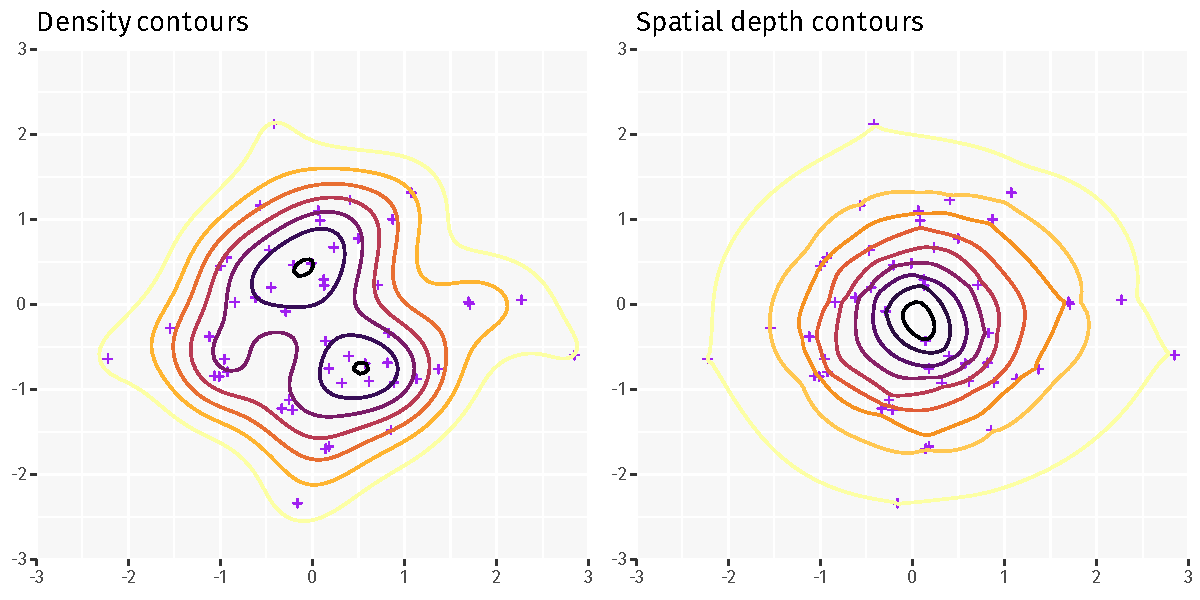
\includegraphics[width = \textwidth, page = 1]{contours_density_depth}
    \caption{
        Density contours (via kernel density estimation) and spatial depth
        (Definition~\ref{def:spatial_depth}) contours for 50 points sampled
        from a standard bivariate normal distribution.
        The depth contours offer a clearer, more robust measure of centrality
        within the data cloud.
    }
    \label{fig:contours_density_depth}
\end{figure}


One method of estimating the density function $f$ from a sample $\{\vx_i\}_{i
= 1}^n$ is via a \emph{kernel density estimator} \parencite{wasserman-2005},
of the form
\begin{equation}
    \hat{f}_{h}(\vx) = \frac{1}{n} \sum_{i = 1}^n K_h(\vx - \vx_i).
\end{equation}
Here, $K_h\colon \R^d \to \R$ is a \emph{kernel function} with
\emph{bandwidth(s)} $h$; a simple example is the Gaussian kernel
\begin{equation}
    K_h(\vz) = \frac{1}{\sqrt{2\pi}\prod_{i = 1}^d h_i}\, \exp\left(-\sum_{i = 1}^d \frac{z_i^2}{2h_i^2}\right)
\end{equation}
The tuning parameters $\{h_i\}_{i = 1}^d$ are typically determined via
cross-validation; an optimal bandwidth is one that minimizes the integrated
risk $\int_{\R^d}\E[(f(\vx) - \hat{f}_h(\vx))^2]\:d\vx$.
It can be shown that under certain circumstances, the integrated risk is of
order $O(n^{-4/(4 + d)})$, which grows swiftly with the dimension $d$.
This in turn means that the number of sample points $n$ required to achieve
the same level of confidence explodes with increasing dimension $d$.
Besides, it is often the case that the number of tuning parameters for the
kernel $K_h$ also increases.
Of course, density estimation in the functional setting is much more complex.
Altogether, density does not provide a tractable quantification of centrality.
Depth functions will turn out to alleviate a majority of these theoretical and
computational concerns.


In Chapter~\ref{chap:multivariate}, we introduce depth functions on
multivariate data and distributions on $\R^d$, with a brief discussion on some
of their properties.
We look at the depth-depth plot as a tool for exploratory data analysis, then
move onto applications in testing, classification, and clustering tasks.
In Chapter~\ref{chap:functional}, we extend our understanding of depth
functions to functional data and distributions on function spaces such as
$L^2$ and $\mathcal{C}$.
We see that although many procedures for multivariate data carry over
naturally to this setting, functional data poses its own unique challenges.
We explore applications of depth functions in classification and outlier
detection tasks, and briefly examine the setting of partially observed data
and the reconstruction problem.
Finally, in Chapter~\ref{chap:localdepth}, we discuss the concept of local
depth, focusing on a general recipe for converting a global depth function
into its local counterpart.
Motivated by the construction of local depth regions, we propose a new kernel
based regression procedure which works reasonably well for univariate,
multivariate, and functional data.


    \section{Centrality vs Density}
    \section{Nonparametric procedures}


    \chapter{Multivariate Data}
    
It is desirable for a depth function $D\colon \R^d \times \mathscr{F} \to \R$
to satisfy the following properties, described by
\textcite{zuo-serfling-2000}.

\begin{enumerate}
    \item[\textbf{P1}.] \emph{Affine invariance.}
        For any random vector $\vX$ in $\R^d$, any $d \times d$ nonsingular
        matrix $A$, and any $d$-vector $\bm{b}$,
        \begin{equation}
            D(A\vx + \bm{b}, F_{A\vX + \bm{b}}) \;=\; D(\vx, F_{\vX}).
        \end{equation}
        This makes $D(\vx, F_{\vX})$ independent of the choice of coordinate
        system.

    \item[\textbf{P2}.] \emph{Maximality at center.}
        For any $F \in \mathscr{F}$ having `center' $\vth$,
        \begin{equation}
            D(\vth, F) \;=\; \sup_{\vx \in \R^d} D(\vx, F).
        \end{equation}
        This means that the deepest point coincides with some center of
        symmetry of the distribution $F$.

    \item[\textbf{P3}.] \emph{Monotonicity relative to deepest point.}
        For any $F \in \mathscr{F}$ having deepest point $\vth$ and for
        $\alpha \in [0, 1]$,
        \begin{equation}
            D(\vx, F) \;\leq\; D(\vth + \alpha(\vx - \vth), F).
        \end{equation}
        Thus, $D(\Cdot, F)$ monotonically decreases along any ray pointing
        away from the deepest point.

    \item[\textbf{P4}.] \emph{Vanishing at infinity.}
        For any $F \in \mathscr{F}$,
        \begin{equation}
            D(\vx, F) \to 0 \quad\text{ as }\quad\norm{\vx} \to \infty.
        \end{equation}
\end{enumerate}

Furthermore, we demand that $D$ be non-negative and bounded.
Thus, we may assume hereon that $D$ only takes values in $[0, 1]$.

The notion of a `center' of a distribution in \textbf{P2} is typically
described in terms of symmetry.
We say that a random vector $\vX$ is \emph{centrally symmetric} about
$\vth \in \R^d$ if $\vX - \vth \eqd \vth - \vX$.
Similarly, we say that $\vX$ is \emph{angularly symmetric} about $\vth$ if
$(\vX - \vth) / \norm{\vX - \vth}$ is centrally symmetric about $\bm0$.
An even more restrictive notion of symmetry is \emph{spherical symmetry},
where we demand that $U(\vX - \vth) \eqd \vX - \vth$ for every orthonormal
matrix $U$.
\emph{Elliptical symmetry} requires that $V\vX$ is spherically symmetric about
$\vth$ for some nonsingular matrix $V$.
Finally, the weakest notions of symmetry discussed here is \emph{halfspace
symmetry}, where we impose $P(\vX \in H) \geq 1/2$ for every closed halfspace
in $\R^d$ containing $\vth$.
Thus, the symmetries in decreasing order of strength are $S > E > C > A > H$.


It is also desirable for a depth function to obey some notions of continuity.
\begin{enumerate}
    \item[\textbf{C1}.] \emph{Continuity in $\vx$.}
    \begin{equation}
        D(\vx_n, F) \to D(\vx, F)\;\text{ when }\; \vx_n \to \vx.
    \end{equation}

    \item[\textbf{C2}.] \emph{Continuity in $F$.}
    \begin{equation}
        D(\vx, F_n) \to D(\vx, F)\;\text{ when }\; F_n \tod F.
    \end{equation}
\end{enumerate}

Property \textbf{C1} is rarely satisfied without imposing some regularity
conditions on $F$, such as absolute continuity.
Property \textbf{C2} helps bridge the gap between the population and empirical
versions of depth.


\section{Multivariate depth functions}

\begin{figure}
    \centering
    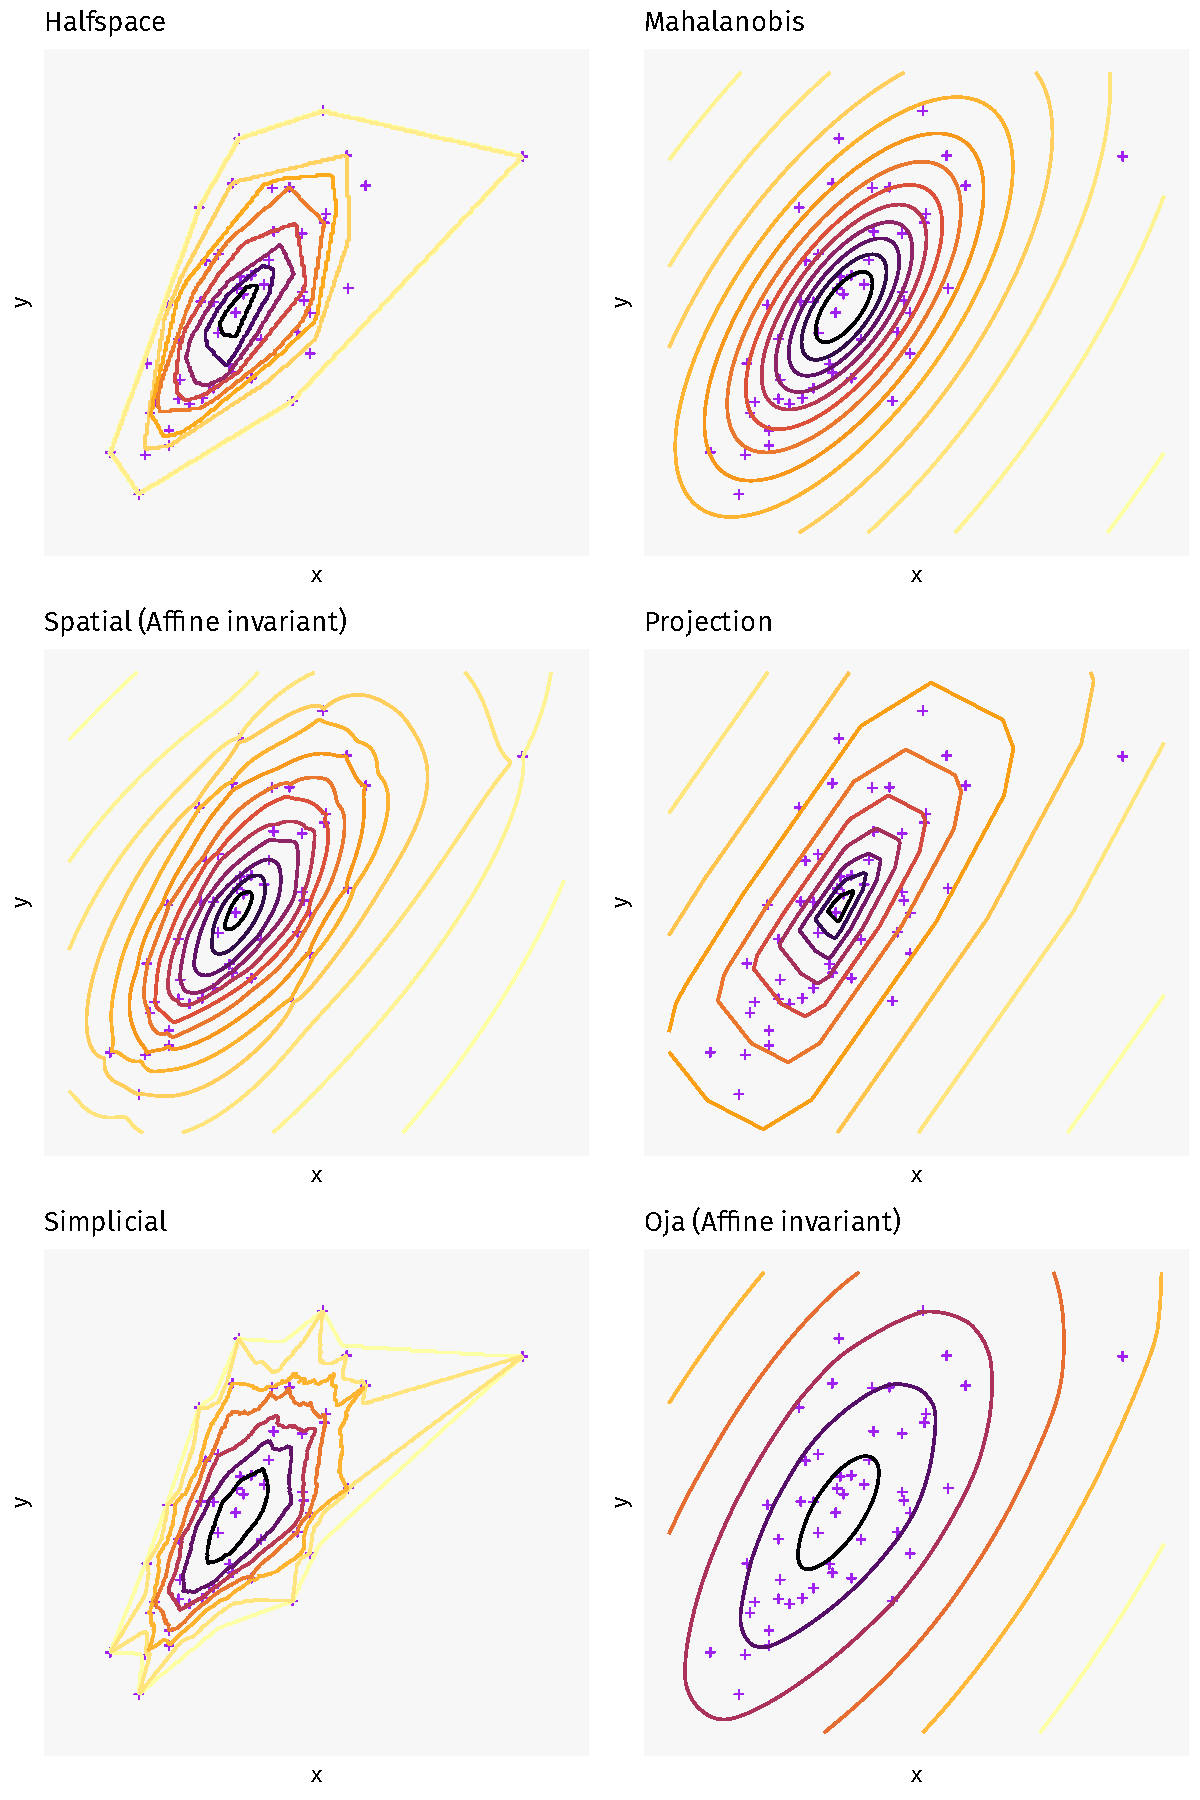
\includegraphics[width = \textwidth, page = 1]{contours}
    \caption{
        Depth contours with respect to purple points.
        Darker contours have higher depth.
    }
    \label{fig:depthcontours}
\end{figure}


The earliest formulation of a depth function may be attributed to
\textcite{tukey-1975}.

\begin{definition}[Halfspace/Tukey depth]
    Denote the collection of all closed halfspaces in $\R^d$ containing $\vx$
    by $\mathcal{H}_{\vx}$.
    The halfspace depth, or Tukey depth, is defined as
    \begin{equation}
        D_H(\vx, F) = \inf_{H \in \mathcal{H}_{\vx}} P_{F}(H).
    \end{equation}
\end{definition}

\begin{remark}
    If $F \in \mathscr{F}$ is supported on a convex region $K \subset \R^d$,
    then $D(\Cdot, F)$ vanishes outside $K$.
    More generally, for convex $K \subset \R^d$, we have $D_H(\vx, F) \leq
    P_F(K^c)$ for all $\vx \in K^c$.
    This is because one can choose a halfspace $H \in \mathcal{H}_{\vx}$
    entirely contained within $K^c$.
    Using this, we see that the halfspace depth obeys \textbf{P4}.
\end{remark}

\begin{proposition}
    The halfspace depth can be formulated as
    \begin{equation}
        D_H(\vx, F) = \inf_{\vv \in S^{d - 1}} P_{\vX \sim F}(\ip{\vv}{\vX} \leq \ip{\vv}{\vx}).
    \end{equation}
\end{proposition}

\begin{remark}
    When $d = 1$, the halfspace depth reduces to
    \begin{equation}
        D_H(x, F) = \min\{P_F(-\infty, x],\, P_F[x, \infty)\}.
    \end{equation}
\end{remark}



\begin{definition}[Mahalanobis depth]
    Let $\vX \sim F$ have mean $\vmu$ and covariance matrix $\Sigma$.
    The Mahalanobis depth is defined as
    \begin{equation}
        D_{M}(\vx, F) = \left(1 + (\vx - \vmu)^\top \Sigma^{-1}(\vx - \vmu)\right)^{-1}.
    \end{equation}
\end{definition}

\begin{remark}
    The mean and covariance in the above definition may be replaced with more
    robust estimates $\vmu^*$ and $\Sigma^*$, for instance using the minimum
    covariance determinant (MCD) method.
    The corresponding depth function is called the robust Mahalanobis depth.
\end{remark}

\begin{definition}[Spatial depth]
    The spatial depth is defined as
    \begin{equation}
        D_{Sp}(\vx, F) = 1 - \left\Vert \E_{\vX \sim F}\left[\frac{\vx - \vX}{\norm{\vx - \vX}}\right] \right\Vert.
    \end{equation}
    We use the convention $\bm0/0 = \bm0$.
\end{definition}

\begin{remark}
    Spatial depth defined as above does not obey \textbf{P1}.
    Indeed, spatial depth is only invariant under spherical transformations of
    the form $U\vX + \bm{b}$ for orthonormal $U$.
    We may define an affine invariant version of spatial depth as
    \begin{equation}
        D_{AISp}(\vx, F) = 1 - \left\Vert \E_{\vX \sim F}\left[\frac{\Sigma^{-1/2}(\vx - \vX)}{\sqrt{(\vx - \vX)^\top\Sigma^{-1}(\vx - \vX)}}\right] \right\Vert.
    \end{equation}
\end{remark}

\begin{remark}
    \textcite{nagy-2017} showed that spatial depth does not obey \textbf{P3}.
\end{remark}


\begin{definition}[Projection depth]
    The projection depth is defined as
    \begin{equation}
        D_P(\vx, F) = \left(1 + \sup_{\vv \in S^{d - 1}} \frac{|\ip{\vv}{\vx} - \med(\ip{\vv}{\vX})|}{\MAD(\ip{\vv}{\vX})}\right)^{-1}, \quad
        \vX \sim F.
    \end{equation}
\end{definition}

\textcite{liu-1990} introduced the following depth function based on random
simplices.

\begin{definition}[Simplicial depth]
    The simplicial depth is defined as
    \begin{equation}
        D_{Sim}(\vx, F) = P_{\vX_i \iid F}(\vx \in \conv(\vX_1, \dots, \vX_{d + 1})),
    \end{equation}
    where $\conv(\vx_1, \dots, \vx_{d + 1})$ denotes the convex hull of
    $\{\vx_1, \dots, \vx_{d + 1}\}$.
\end{definition}

\begin{definition}[Oja depth]
    The simplicial volume depth, or Oja depth, is defined as
    \begin{equation}
        D_{Oja}(\vx, F) = \left(1 + \E_{\vX_i \iid F}\left[\vol(\conv(\vx, \vX_1, \dots, \vX_d))\right]\right)^{-1}.
    \end{equation}
\end{definition}

\begin{remark}
    Oja depth does not obey \textbf{P1}, since
    \begin{equation}
        \vol(\conv(A\vx_1 + \bm{b}, \dots, A\vx_{d + 1} + \bm{b})) = |\det(A)| \vol(\conv(\vx_1, \dots, \vx_{d + 1})).
    \end{equation}
    Instead, we may define an affine invariant version of Oja depth as
    \begin{equation}
        D_{AIOja}(\vx, F) = \left(1 + \E_{\vX_i \iid F}\left[\frac{\vol(\conv(\vx, \vX_1, \dots, \vX_d))}{\sqrt{\det(\Sigma)}}\right]\right)^{-1},
    \end{equation}
    where $\Sigma$ is the covariance matrix of $F$.
\end{remark}


\begin{remark}
    The Mahalanobis, projection, and Oja depths all follow the pattern of $(1
    + O(\vx, F))^{-1}$, where $O(\vx, F)$ measures some kind of outlyingess of
    $\vx$ in $F$.
    We will often see this performed in reverse, extracting a measure of
    outlyingess $1/D(\vx, F) - 1$ from a depth function $D$.
\end{remark}


\subsection{The projection property}


\begin{definition}[Projection property]
    We say that a depth function $D$ has the projection property if
    \begin{equation}
        D(\vx, F_{\vX}) = \inf_{\vv \in S^{d - 1}} D(\ip{\vv}{\vx}, F_{\ip{\vv}{\vX}}).
    \end{equation}
\end{definition}

Depths which have this property can be approximated by calculating the
univariate depths of the projected data along many directions $\vv$.


\begin{lemma}[\cite{mosler-mozharovskyi-2022}]
    The halfspace depth, Mahalanobis depth, and projection depth have the
    projection property.
\end{lemma}

The halfspace depth in particular is often computationally challenging.
Thus, the property motivates the definition of the random Tukey depth
\parencite{albertos-reyes-2008a}.

\begin{definition}[Random Tukey depth]
    Let $\vv_1, \dots, \vv_n$ be a realization of an iid sample from $\UU(S^{d
    - 1})$.
    The random Tukey depth is defined as
    \begin{equation}
        D_{RT}(\vx, F_{\vX}) = \min_{1 \leq i \leq n} D_H(\ip{\vv_i}{\vx}, F_{\ip{\vv_i}{\vX}}).
    \end{equation}
\end{definition}



\subsection{Continuity properties}

It is also desirable for a depth function to obey some notions of continuity.
\begin{enumerate}
    \item[\textbf{C1}.] \emph{Continuity in $\vx$.}
    \begin{equation}
        D(\vx_n, F) \to D(\vx, F)\;\text{ when }\; \vx_n \to \vx.
    \end{equation}

    \item[\textbf{C2}.] \emph{Continuity in $F$.}
    \begin{equation}
        D(\vx, F_n) \to D(\vx, F)\;\text{ when }\; F_n \tod F.
    \end{equation}

    \item[\textbf{C3}.] \emph{Uniform continuity}.
    \begin{equation}
        \sup_{\vx \in G} |D(\vx, F_n) - D(\vx, F)| \to 0\;\text{ when }\; F_n \tod F.
    \end{equation}
\end{enumerate}

Property \textbf{C1} is rarely satisfied without imposing some regularity
conditions on $F$, such as absolute continuity.
Property \textbf{C2} helps bridge the gap between the population and empirical
versions of depth.
Property \textbf{C3} becomes relevant when dealing with the convergence of
depth contours.


The Mahalanobis depth is trivially continuous in $\vx$, i.e.\ obeys
\textbf{C1}.
Furthermore, it also satisfies \textbf{C2} as long as $F$ has a regular
covariance matrix \parencite{mosler-mozharovskyi-2022}.


The halfspace depth also enjoys all three notions of continuity, under mild
restrictions on $F$.

\begin{theorem}[\cite{mizera-volauf-2002}]
    Let $F \in \mathscr{F}$ be such that the probability of every hyperplane
    in $\R^d$ is zero, i.e.\ for all $\alpha \in \R$ and $\vv \in S^{d - 1}$,
    \begin{equation}
        P_{\vX \sim F}(\ip{\vv}{\vX} = \alpha) \;=\; 0. \label{eq:halfspace_continuity}
    \end{equation}
    Then for $\vx_n \to \vx$ and $F_n \tod F$, we have $D_H(\vx_n, F_n) \to
    D_H(\vx, F)$.
\end{theorem}
\begin{remark}
    Equation~\ref{eq:halfspace_continuity} is satisfied whenever $F$ is
    absolutely continuous.
\end{remark}
\begin{remark}
    It follows that if $F \in \mathscr{F}$ satisfies
    Equation~\ref{eq:halfspace_continuity}, then the map $D_H(\Cdot, F)$ is
    continuous.
\end{remark}

\begin{corollary}
    Let $F \in \mathscr{F}$ satisfy Equation~\ref{eq:halfspace_continuity}.
    Then, for $F_n \tod F$, and compact $K \subset \R^d$,
    \begin{equation}
        \sup_{\vx \in K} |D_H(\vx, F_n) - D_H(\vx, F)| \to 0.
    \end{equation}
\end{corollary}
\begin{proof}
    Denoting $g = D(\Cdot, F)$, $g_n = D_H(\Cdot, F_n)$, we have the
    continuity of $g$ along with $g_n(\vx_n) \to g(\vx)$ whenever $\vx_n \to
    \vx$ in $K$.
    If the given conclusion is false, we may pass to a subsequence of $g_n$
    and find $\epsilon > 0$ such that each $\sup_{\vx \in K} |g_n(\vx) -
    g(\vx)| \geq \epsilon$.
    Using the compactness of $K$, we pass to a further subsequence and find
    $\vx \in K$ such that $\vx_n \to \vx$.
    This contradicts $|g_n(\vx_n) - g(\vx_n)| \geq \epsilon$.
\end{proof}

\begin{theorem}\label{thm:halfspace_uniform}
    Let $F \in \mathscr{F}$ satisfy Equation~\ref{eq:halfspace_continuity}.
    Then, for $F_n \tod F$,
    \begin{equation}
        \sup_{\vx \in \R^d} |D_H(\vx, F_n) - D_H(\vx, F)| \to 0.
    \end{equation}
\end{theorem}
\begin{proof}
    Let $K_r = \{\vx \in \R^d\colon \norm{\vx} \leq r\}$ be a continuity set
    of $F$.
    Observe that $D_H(\vy, F) \leq P_F(K_r^c)$ for $\vy \in K_r^c$, hence
    \begin{equation}
        \sup_{\vy \in K_r^c} |D_H(\vy, F_n) - D_H(\vy, F)| \leq P_{F_n}(K_r^c) + P_F(K_r^c).
    \end{equation}
    As $n \to \infty$, we have $P_{F_n}(K_r^c) \to P_F(K_r^c) = p_r$ (say).
    Thus, denoting $\delta_n(X) = \sup_{\vx \in X} |D_H(\vx, F_n) - D_H(\vx,
    F)|$, we have
    \begin{align}
        \limsup_{n \to \infty} \delta_n(\R^d)
        &\leq \lim_{n \to \infty} \delta_n(K_r) + \limsup_{n \to \infty} \delta_n(K_r^c) \\
        &\leq 0 + 2p_r.
    \end{align}
    Using $p_r \to 0$ as $r \to \infty$ completes the proof.
\end{proof}



The spatial depth is similarly well behaved.

\begin{theorem}
    Spatial depth obeys \textbf{C1} when $F$ is non-atomic, as well as
    \textbf{C2}.
\end{theorem}
\begin{proof}
    Consider the spatial map
    \begin{equation}
        S_F\colon \R^d \to \R^d, \qquad
        \vx \mapsto \E_{\vX \sim F}\left[\frac{\vx - \vX}{\norm{\vx - \vX}}\right].
    \end{equation}
    The Dominated Convergence Theorem guarantees the continuity of $S_F$,
    hence of $D_{Sp}(\Cdot, F) = 1 - \norm{S_F(\Cdot)}$.
    Furthermore, if $F_n \tod F$, we have $S_{F_n}(\vx) \to S_F(\vx)$ by the
    Portmanteau Lemma for all $\vx \in \R^d$.
\end{proof}

\begin{theorem}[\cite{serfling-2002}]
    For $F \in \mathscr{F}$ and compact $K \subset \R^d$,
    \begin{equation}
        \sup_{\vx \in K} |D_{Sp}(\vx, \hat{F}_n) - D_{Sp}(\vx, F)| \toas 0.
    \end{equation}
\end{theorem}

\begin{remark}
    This result can be generalized from compact subsets $K$ to the whole of
    $\R^d$, using the following Lemma (\ref{lem:spatial_vanish}) and arguments
    similar to the proof of Theorem~\ref{thm:halfspace_uniform}.
\end{remark}

\begin{lemma}\label{lem:spatial_vanish}
    Spatial depth obeys \textbf{P4}, i.e.\ $D_{Sp}(\vx, F) \to 0$ as
    $\norm{\vx} \to \infty$.
\end{lemma}
\begin{proof}
    Let $\epsilon > 0$, and let $M > 0$ such that $P_{\vX \sim F}(\norm{\vX} >
    M) = \epsilon$.
    Denote $\vY = (\vx - \vX) / \norm{\vx - \vX}$, and observe that
    \begin{equation}
        \E_{\vX \sim F}\left[\vY\right]
        = (1 - \epsilon)\E\left[\vY|\, \norm{\vX} \leq M\right] +
          \epsilon\E\left[\vY|\, \norm{\vX} > M\right]
    \end{equation}
    Thus, using $\norm{\vY} = 1$ and the reverse triangle inequality,
    \begin{equation}
        \norm{\E\left[\vY\right]}
        \geq (1 - \epsilon)\norm{\E\left[\vY|\, \norm{\vX} \leq M\right]} - \epsilon.
    \end{equation}
    Let $\alpha = \arccos((1 - 2\epsilon)/(1 - \epsilon))$, and let $r_\alpha =
    M/\sin\alpha$.
    It follows that the ball $\{\vx \in \R^d\colon \norm{\vx} \leq M\}$
    subtends an angle of at most $2\alpha$ from any point $\vx$ such that
    $\norm{\vx} > r_\alpha$.
    This gives $\norm{\E[\vY \mid \norm{\vX} \leq M]} \geq \cos\alpha$.
    Thus, for $\norm{\vx} > r_\alpha$,
    \begin{equation}
        \norm{\E[\vY]} \geq (1 - \epsilon)\cos\alpha - \epsilon = 1 - 3\epsilon,
    \end{equation}
    whence $D_{Sp}(\vx, F) \leq 3\epsilon$.
\end{proof}



\subsection{Characterization properties}

It seems natural to ask the question -- do depth functions completely
characterize a distribution, the way density functions do?
In other words, can we recover $F \in \mathscr{F}$ from $D(\Cdot, F)$?
For most depth functions, the answer is `no', unless we greatly restrict the
class of functions $\mathscr{F}$ under consideration.
For instance, the Mahalanobis depth $D_M(\Cdot, F)$ only depends on the first
two moments of $F$, and thus has no hope of distinguishing between
distributions which differ in higher moments.
On the other hand, if we only consider a family of elliptical distributions
$\Ell(h; \Cdot, \Cdot)$ for strictly monotonically decreasing $h$, it can be
shown that any depth $D$ satisfying \textbf{P1} and \textbf{C1} uniquely
determines $F$ \parencite{mosler-mozharovskyi-2022}.


\begin{definition}[Elliptical distributions]
    \label{def:elliptical}
    We say that a distribution is elliptical if it has a density of the form
    \begin{equation}
        f(\vx) = c\, |\Sigma|^{-1/2}\, h\left((\vx - \vmu)^\top \Sigma^{-1} (\vx - \vmu)\right)
    \end{equation}
    for some non-increasing function $h$.
    This is denoted by $\Ell(h; \vmu, \Sigma)$.
\end{definition}


A positive result for the halfspace depth is that it fully characterizes
empirical distributions.

\begin{theorem}[\cite{struyf-rousseeuw-1999}]
    The empirical distribution of any dataset $\{\vX_i\}_{i = 1}^n \subset
    \R^d$ is uniquely determined by its halfspace depth function $D(\Cdot,
    \hat{F}_n)$.
\end{theorem}

\textcite{nagy-2020} offers a comprehensive overview of the halfspace depth
characterization problem.
Indeed, \textcite{nagy-2021} supplies examples of distinct probability
distributions $F_1, F_2$ such that $D_H(\Cdot, F_1) = D_H(\Cdot, F_2)$.
It can be shown that for an $\alpha$-symmetric distribution $F$ that $D_H(\vx,
F) = G(-\norm{\vx}_{\alpha^*})$, where $G$ is the marginal distribution of the
first component of $\vX \sim F$ and $1/\alpha + 1/\alpha^* = 1$.




\section{Depth contours}
\label{sec:multivariate_depthcontours}

Given a depth function $D$ and some fixed distribution $F \in \mathscr{F}$, we
may examine contours produced by $D(\Cdot, F)$.
The following definitions are adapted from \cite{liu-parelius-singh-1999}.

\begin{definition}
    The contour of depth $t$ is the set $\{\vx \in \R^d : D(\vx, F) = t\}$.
\end{definition}

\begin{definition}
    The region enclosed by the contour of depth $t$ is the set
    \begin{equation}
        R_F(t) \,=\, \{\vx \in \R^d : D(\vx, F) > t\}.
    \end{equation}
\end{definition}

It is often more convenient to deal with depth contours and regions based on
their probability content rather than a depth cutoff.

\begin{definition}
    The $p$-th central region is the set
    \begin{equation}
        C_F(p) \,=\, \bigcap_{t}\; \{R_F(t) : P_F(R_F(t)) \geq p\}.
    \end{equation}
\end{definition}

\begin{definition}
    The $p$-th level contour, or center-outward contour surface, is the set
    $Q_F(p) = \partial C_F(p)$.
\end{definition}


\begin{example}
    Consider $\UU(B^d)$, i.e.\ the uniform distribution on the unit ball in
    $\R^d$.
    While there are no proper density contours to speak of, halfspace depth
    contours are concentric spheres centered at the origin, the deepest point.
    This illustrates how depth contours are more suited to indicating
    centrality than density contours.
\end{example}


\begin{definition}
    Let $\vX_1, \dots, \vX_n \iid F$.
    We introduce depth based order statistics $\vX_{[1]}, \dots, \vX_{[n]}$,
    which are a reordering of the sample in decreasing order of depth, i.e.\
    $D(\vX_{[1]}, F) \geq \dots \geq D(\vX_{[n]}, F)$.
\end{definition}

With this, given $\vX_1, \dots, \vX_n \iid F$, the sample $p$-th central
region is given by
\begin{equation}
    C_{\hat{F}_n}(p) = \conv(\vX_{[1]}, \dots, \vX_{[\lceil np \rceil]}).
\end{equation}


\section{Depth-Depth plots}

\begin{definition}[DD plot] \label{def:ddplot}
    Let $F, G$ be two distributions on $\R^d$, and let $D$ be a depth
    function. The Depth-Depth plot, also known as the DD plot, of $F$ and $G$
    is given by
    \begin{equation}
        \DD(F, G) \,=\, \{(D(\vz, F), D(\vz, G)) : \vz \in \R^d\}.
    \end{equation}
\end{definition}
\begin{remark}
    The above definition generalizes naturally to involve more than two
    distributions on $\R^d$.
\end{remark}

When the depth function $D$ only takes values in $[0, 1]$, the DD plot is a
subset of $[0, 1]^2$ and hence easily visualized.
Clearly when $F = G$, the corresponding DD plot is confined to the diagonal
$\{(t, t) : t \in [0, 1]\}$.
However, when $d \geq 2$ and $F, G$ are absolutely continuous, $\DD(F, G)$ has
non-zero area (Lebesgue measure) when $F \neq G$.
Assuming that $D$ is affine invariant, \textcite{liu-parelius-singh-1999}
propose this area as an affine invariant measure of the discrepancy between
$F$ and $G$.



\begin{figure}
    \centering
    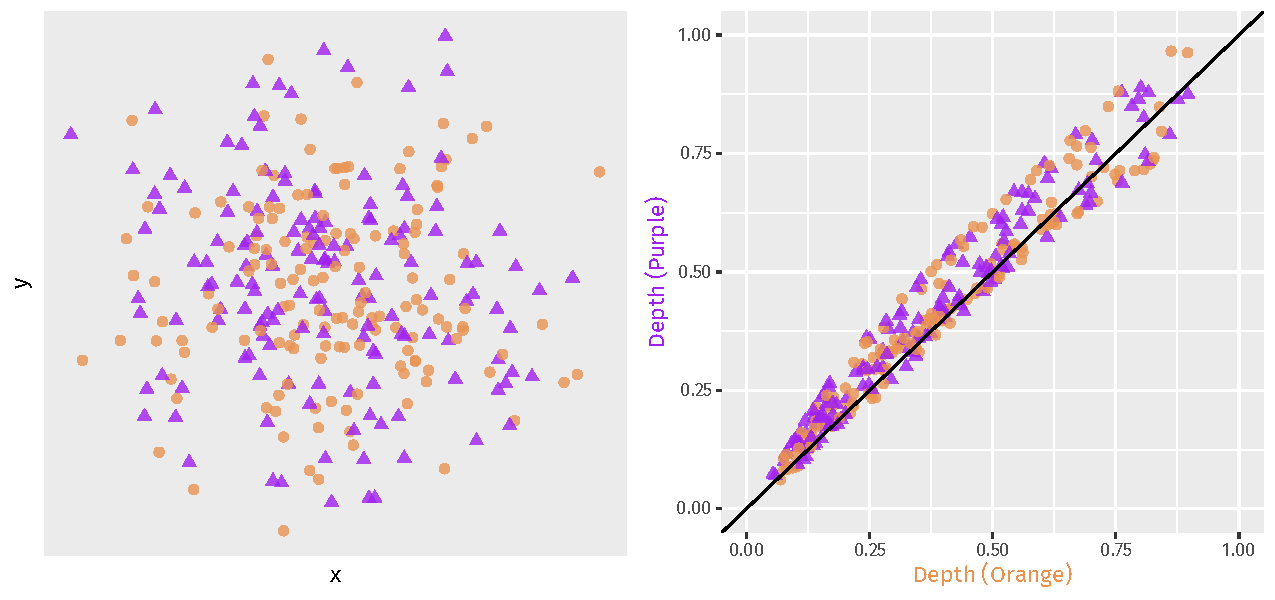
\includegraphics[width = \textwidth, page = 1]{ddplots}
    \caption{
        Empirical DD plot using spatial depth, where both underlying
        distributions (bivariate normal) are identical.
        Observe how the points in the DD plot stay close to the diagonal black
        line.
    }
    \label{fig:ddplots_identical}
\end{figure}



If the distributions $F, G$ are unknown, we may use data samples
$\mathscr{D}_F = \{\vX_i\}$ and $\mathscr{D}_G = \{\vY_j\}$ where $\vX_1,
\dots, \vX_n \iid F$ and $\vY_1, \dots, \vY_m \iid G$, then construct
empirical distributions $\hat{F}_n, \hat{G}_m$.
With this, we may examine the empirical DD plot
\begin{equation}
    \DD(\hat{F}_n, \hat{G}_n) \,=\, \{(D(\vz, \hat{F}_n), D(\vz, \hat{G}_m)) : \vz \in \mathscr{D}_F \cup \mathscr{D}_G\}.
\end{equation}

DD plots can be used as a diagnostic tool to detect differences in location
and scale between two multivariate distributions.
\begin{enumerate}[itemsep=0em]
    \item If $F = G$, the points in $\DD(\hat{F}_n, \hat{G}_m)$ stay close to
    the diagonal.
    See Figure~\ref{fig:ddplots_identical}.

    \item If the same point $\vz_0$ achieves maximum depths with respect to
    both distributions $F$ and $G$, this indicates that $\vz_0$ is their
    common center.
    See Figure~\ref{fig:ddplots_location}.

    \item Suppose that $F$ and $G$ have the same center. If the points in
    $\DD(\hat{F}_n, \hat{G}_m)$ arch above the diagonal, i.e.\ the bulk of
    points are deeper in $G$ than in $F$, this indicates that $F$ has a
    greater spread than $G$.
    See Figure~\ref{fig:ddplots_scale_a}.
\end{enumerate}

\textcite{liu-parelius-singh-1999} also demonstrate the use of DD plots to
detect differences in skewness and kurtosis.
This tool is especially convenient since the DD plot is always two dimensional
regardless of the dimension $d$ of the sample points.


\begin{figure}
    \centering
    \includegraphics[width = \textwidth, page = 2]{ddplots}
    \caption{
        Empirical DD plot using spatial depth, where both underlying
        distributions (bivariate normal) differ only in location.
        Observe how most of the orange points fall in the lower triangle,
        while the purple ones fall in the upper triangle.
        The deepest point with respect to the orange distribution has fairly
        low depth with respect to the purple one, and vice versa.
    }
    \label{fig:ddplots_location}
\end{figure}



\begin{figure}
    \centering
    \begin{subfigure}[b]{\textwidth}
        \centering
        \includegraphics[width = \textwidth, page = 3]{ddplots}
        \subcaption{
            $
                \textcolor{Orange}{\Sigma_+} = \I_2, \quad
                \textcolor{Purple}{\Sigma_\times} = 4\I_2,
            $
        }
        \label{fig:ddplots_scale_a}
    \end{subfigure}
    \\[1em]
    \begin{subfigure}[b]{\textwidth}
        \centering
        \includegraphics[width = \textwidth, page = 4]{ddplots}
        \subcaption{
            $
            \textcolor{Orange}{\Sigma_+} = \begin{bmatrix}
                1 & -0.5 \\ -0.5 & 1
            \end{bmatrix}, \quad
            \textcolor{Purple}{\Sigma_\times} = \begin{bmatrix}
                1 & 0.5 \\ 0.5 & 1
            \end{bmatrix}.
            $
        }
        \label{fig:ddplots_scale_b}
    \end{subfigure}
    \\[1em]
    \caption{
        Empirical DD plot using spatial depth, where both underlying
        distributions (bivariate normal) differ only in scale.
        In \textbf{(a)}, observe how the points remain in the upper triangle
        in the DD plot.
        In \textbf{(b)}, observe how there are more orange points in the lower
        triangle, and more purple points in the upper triangle in the DD plot,
        especially in the region close to the origin.
    }
    \label{fig:ddplots_scale}
\end{figure}



\begin{figure}
    \centering
    \includegraphics[width = \textwidth, page = 5]{ddplots}
    \caption{
        Empirical DD plot using spatial depth, where both underlying
        distributions (bivariate normal) differ in both location and scale.
        Observe that there is a clear separation between the orange and purple
        points in the DD plot, although not about the diagonal line.
    }
    \label{fig:ddplots_location_scale}
\end{figure}



\section{Testing}

We are mainly interested in the two sample homogeneity test.
Given samples from $F$ and $G$, we wish to test the null hypothesis $H_0: F =
G$ against an alternate hypothesis that $F$ and $G$ differ in location or
scale.

When $F, G$ are distributions on $\R$, rank based tests such as the Wilcoxon
rank-sum test or the Siegel-Tukey test are readily available.
A very useful tool in this setting is the probability integral transform.

\begin{proposition}
    Let $\vX \sim F$, and let the distribution $F$ be continuous.
    Then, $F(\vX) \sim \UU[0, 1]$.
\end{proposition}

Since $F(\vX_j)$ has the same rank within $\{F(\vX_i)\}$ as does $\vX_j$
within $\{\vX_i\}$, the above result is the key towards establishing many
distribution-free tests and procedures.


In the multivariate setting, \textcite{liu-singh-1993} use the following depth
based analogue.

\begin{definition}
    Denote
    \begin{equation}
        R(\vz, F) = P(D(\vX, F) \leq D(\vz, F) \mid \vX \sim F).
    \end{equation}
\end{definition}

Note that in the empirical setting, $R(\vz, \hat{F}_n)$ is simply the
proportion of sample points $\{\vX_i\}$ which are deeper in $F$ than $\vz$.


\begin{proposition}[\cite{liu-singh-1993}]
    Let $\vX \sim F$, and let the distribution of $D(\vX, F)$ be continuous.
    Then, $R(\vX, F) \sim \UU[0, 1]$.
\end{proposition}


\begin{definition}
    Denote the quality index
    \begin{equation}
        Q(F, G) = P(D(\vX, F) \leq D(\vY, F) \mid \vX \sim F,\, \vY \sim G).
    \end{equation}
\end{definition}

Note that $Q(F, G)$ and $Q(G, F)$ are not necessarily the same.
We may also write
\begin{equation}
    Q(F, G) = \E_{\vY \sim G}[R(\vY, F)].
\end{equation}


It is clear that $Q(F, G) = 1/2$ when $F = G$.
It can be shown under special circumstances that $Q(F, G) < 1/2$ if $F, G$
differ in terms of location or scale.
This will form the basis of our testing scheme, with $H_0: F = G$ versus $H_A:
Q(F, G) < 1/2$.

Here, we restrict our attention to elliptical distributions on $\R^d$.

\begin{definition}[Elliptical distributions]
    We say that a distribution is elliptical if it has a density of the form
    \begin{equation}
        f(\vx) = c\, |\Sigma|^{-1/2}\, h\left((\vx - \vmu)^\top \Sigma^{-1} (\vx - \vmu)\right)
    \end{equation}
    for some non-increasing function $h$.
    This is denoted by $\Ell(h; \vmu, \Sigma)$.
\end{definition}

% \begin{proposition}[\cite{liu-singh-1993}]
%     Let $F \sim \Ell(h; \vmu, \Sigma)$ and $G_t \sim \Ell(h; \vmu +
%     t\hat{\vv}, \Sigma)$ for some unit vector $\hat{\vv}$ and $t \geq 0$.
%     Further suppose that $D(\cdot, F)$ has the affine invariance and
%     monotonicity properties.
%     Then, $Q(F, G_t)$ is non-increasing with increasing $t$.
% \end{proposition}

% \begin{proposition}[\cite{liu-singh-1993}]
%     Let $F \sim \Ell(h; \vmu, \Sigma_1)$ and $G \sim \Ell(h; \vmu, \Sigma_2)$
%     where $\Sigma_1 - \Sigma_2$ is positive definite.
%     Further suppose that $D(\cdot, F)$ has the affine invariance property.
%     Then, $Q(F, G) \leq 1/2$.
% \end{proposition}

The quality index obeys the following properties.

\begin{proposition}[\cite{liu-singh-1993}]
    Let $F \sim \Ell(h; \vmu_1, \Sigma_1)$ and $G \sim \Ell(h; \vmu_2,
    \Sigma_2)$ where $\Sigma_1 - \Sigma_2$ is positive definite.
    Further suppose that $D(\cdot, F)$ has the affine invariance and
    monotonicity properties.
    Then, $Q(F, G) \leq 1/2$ decreases monotonically as $\vmu_2$ is moved away
    from $\vmu_1$ along any line.
\end{proposition}

\begin{proposition}[\cite{liu-singh-1993}]
    Let $F \sim \Ell(h; \vmu, \Sigma_1)$ and $G \sim \Ell(h; \vmu,
    \Sigma_2)$ where $\Sigma_1 - \Sigma_2$ is positive definite.
    Consider Huber's contamination of the form
    \begin{equation}
        G_\alpha = (1 - \alpha)F + \alpha G
    \end{equation}
    where $0 \leq \alpha \leq 1$.
    Then, $Q(F, G_\alpha)$ decreases monotonically as $\alpha$ increases.
\end{proposition}

This motivates a modified Wilcoxon rank-sum test in the multivariate setting,
using the quality index $Q(F, G)$.
Let $\vX_1, \dots, \vX_n \iid F$, and $\vY_1, \dots, \vY_m \iid G$.
Since $R(\cdot, F), Q(F, \cdot)$ depend on $D(\cdot, F)$, the latter has to be
approximated using $D(\cdot, \hat{F}_{n_0})$, where $\hat{F}_{n_0}$ is based
on a (fairly large) additional sample $\vZ_1, \dots, \vZ_{n_0} \iid F$, with
$n_0 \gg n, m$.
With this, we compute
\begin{equation}
    R(\,\cdot\,, \hat{F}_{n_0}) = \frac{1}{n_0} \sum_{i = 1}^{n_0} \bm{1}(D(\vZ_i, \hat{F}_{n_0}) \leq D(\,\cdot\,, \hat{F}_{n_0})).
\end{equation}
Assign ranks $1, \dots, n + m$ to the arranged values $R(\vX_i,
\hat{F}_{n_0}), R(\vY_j, \hat{F}_{n_0})$ (ascending order), and define $W$ to
be the sum of ranks of the $R(\vY_j, \hat{F}_{n_0})$.
If necessary, break ties at random.
Under the null hypothesis $F = G$, it is clear that $W$ has the same
distribution as the sum of $m$ numbers drawn without replacement from $\{1,
\dots, n + m\}$.
Under the alternate hypothesis $Q(F, G) < 1/2$, the ranks of $R(\vY_j,
\hat{F}_{n_0})$ will tend to be lower on average, making $W$ smaller.

\begin{theorem}[\cite{liu-singh-1993}]
    Let $H_{n, m}$ be the distribution of the sum of $m$ numbers drawn
    randomly without replacement from $\{1, \dots, n + m\}$.
    Suppose that $F$ admits a density function $f$.
    Under the null hypothesis $F = G$, we have $W \sim H_{n, m}$.
\end{theorem}

It is also possible to approximate $Q(F, G)$ more directly via $Q(\hat{F}_n,
\hat{G}_m)$ and perform our test this way.
This sidesteps the need for the `reference' sample $\vZ_1, \dots, \vZ_{n_0}
\iid F$.
Note that
\begin{equation}
    Q(\hat{F}_n, \hat{G}_m)
    = \frac{1}{m}\sum_{j = 1}^m R(\vY_j, \hat{F}_n)
    = \frac{1}{nm}\sum_{i, j} \bm{1}(D(\vX_i, \hat{F}_n) \leq D(\vY_j, \hat{F}_n)).
\end{equation}
This estimate is indeed consistent under mild assumptions.

\begin{theorem}[\cite{liu-singh-1993}]
    Suppose that the distribution of $D(\vY, F)$ is continuous where $\vY \sim
    G$, and that
    \begin{equation}
        \sup_{\vz \in \R^d} |D(\vz, \hat{F}_n) - D(\vz, F)| \toas 0.
    \end{equation}
    Then, $Q(\hat{F}_n, \hat{G}_n) \toas Q(F, G)$ as $\min\{n, m\} \to
    \infty$.
\end{theorem}

This allows us to determine the asymptotic null distribution of $Q(\hat{F}_n,
\hat{G}_m)$.

\begin{theorem}[\cite{liu-singh-1993}]
    Let $F$ be absolutely continuous, such that $\E_{\vX \sim F} \norm{\vX}^4
    < \infty$.
    Using Mahalanobis depth to define $Q$, we have
    \begin{equation}
        S(\hat{F}_n, \hat{G}_m) = \left[\frac{1}{12}\left(\frac{1}{n} + \frac{1}{m}\right)\right]^{-1/2} \left[Q(\hat{F}_n, \hat{G}_m) - \frac{1}{2}\right] \tod \NN(0, 1)
    \end{equation}
    as $\min\{n, m\} \to \infty$, under the null hypothesis $F = G$.
\end{theorem}

Observe that given two samples, we have a choice between using $Q(\hat{F}_n,
\hat{G}_m)$ or $Q(\hat{G}_m, \hat{F}_n)$.
\textcite{shi-zhang-fu-2023} propose a weighted combination of the form
\begin{equation}
    W^\alpha_{n, m} = \alpha S(\hat{F}_n, \hat{G}_m)^2 + (1 - \alpha) S(\hat{G}_m, \hat{F}_n)^2
\end{equation}
for $\alpha \in [0, 1]$, or a maximum
\begin{equation}
    M_{n, m} = \max\{S(\hat{F}_n, \hat{G}_m)^2, S(\hat{G}_m, \hat{F}_n)^2\}.
\end{equation}
Under similar assumptions, they show that both $W^\alpha_{n, m} \tod \chi^2_1$
and $M_{n, m} \tod \chi^2_1$ as $\min\{n, m\} \to \infty$ and $n / m$
converges to a positive constant, under the null hypothesis $F = G$.


\section{Classification}
\label{ch:multivariate_classification}

The $k$-class classification task involves assigning an observation $\vx$ to
one of $k$ populations, described by distributions $F_i$ for $1 \leq i \leq
k$.
The populations may also be associated with prior probabilities $\pi_i$.

\begin{definition}[Classifier]
    A classifier is a map $\hat{\iota}\colon \R^d \to \{1, \dots, k\}$.
\end{definition}

\begin{example}[Bayes classifier]
    Suppose that the population densities $f_i$ for each $1 \leq i \leq k$ are
    known.
    The Bayes classifier assigns $\vx$ to the $\hat{\iota}_B$-th population
    where
    \begin{equation}
        \hat{\iota}_B(\vx) \,=\, \argmax_{1 \leq i \leq k}\; \pi_i f_i(\vx).
    \end{equation}
\end{example}

One way of measuring the performance of a classifier (given the population
distributions and their priors) is by measuring its average misclassification
rate.

\begin{definition}[Average misclassification rate]
    The average misclassification rate of a classifier $\hat{\iota}$ is given
    by
    \begin{equation}
        \Delta(\hat{\iota}) \,=\, \sum_{i = 1}^k \pi_i P(\hat{\iota}(\vX) \neq i \mid \vX \sim F_i).
    \end{equation}
\end{definition}

\begin{proposition}
    The Bayes classifier has the lowest possible average misclassification
    rate. This is known as the optimal Bayes risk, denoted $\Delta_B$.
\end{proposition}

The simplest depth based classifier is the maximum depth classifier
\parencite{ghosh-chaudhuri-2005}.

\begin{example}[Maximum depth classifier]
    Suppose that the prior probabilities $\pi_i$ are equal.
    The maximum depth classifier $\hat{\iota}_D$ for a choice of depth
    function $D$ is described by
    \begin{equation}
        \hat{\iota}_D(\vx) \,=\, \argmax_{1 \leq i \leq k}\; D(\vx, F_i).
    \end{equation}
\end{example}

In practice, instead of having direct access to the population distributions
$F_i$, we have typically deal with labeled training data
\begin{equation}
    \mathscr{D} \,=\, \{(\vx_{ij}, i)\} \subset \R^d \times \{1, \dots, k\},
\end{equation}
where $\vx_{i1}, \dots, \vx_{in_i} \iid F_i$ for each $1 \leq i \leq k$.
The empirical maximum depth classifier simply replaces the population
distributions $F_i$ with their empirical counterparts $\hat{F}_i$ determined
by $\vx_{i1}, \dots, \vx_{in_i}$. Thus, it is given by
\begin{equation}
    \hat{\iota}_{D}(\vx) \,=\, \argmax_{1 \leq i \leq k}\; D(\vx, \hat{F}_i).
\end{equation}
Under certain restrictions, this classifier becomes asymptotically optimal in
the following sense.

\begin{theorem}[\cite{ghosh-chaudhuri-2005}]
    Suppose that the population density functions $f_i$ are elliptically
    symmetric, with $f_i(\vx) = g(\vx - \vmu_i)$ for parameters $\vmu_i$ and a
    density function $g$ such that $g(k\vx) \leq g(\vx)$ for every $\vx$ and
    $k > 1$. Further suppose that the priors on the populations are equal, and
    the depth function $D$ is one of HD, SD, MJD, PD. Then,
    $\Delta(\hat{\iota}_{D}) \to \Delta_B$ as $\min\{n_1, \dots,
    n_k\} \to \infty$.
\end{theorem}

Note that this result deals with elliptic population densities differing only
in location.
Relax this assumption, and instead suppose that $f_i \sim \Ell(h_i; \vmu_i,
\Sigma)$, i.e.
\begin{equation}
    f_i(\vx) = c_i |\Sigma|^{-1/2} h_i\left((\vx - \vmu_i)^\top \Sigma^{-1} (\vx - \vmu_i)\right)
\end{equation}
for strictly decreasing $h_i$, and that the depths can be expressed as
$D(\Cdot, F_i) = l_i(f_i(\Cdot))$ for strictly increasing functions $l_i$.
It follows that the Bayes decision rule can be reformulated as
\begin{equation}
    \pi_i f_i(\vx) > \pi_j f_j(\vx) \;\iff\; D(\vx, F_i) > r_{ij}(D(\vx, F_j))
\end{equation}
for some real increasing function $r_{ij}$.
Using this observation, the DD classifier \parencite{li-albertos-liu-2012}
picks separating functions $r_{ij}$ which best classify the training data
$\mathscr{D}$.

\begin{definition}[Empirical misclassification rate]
    The empirical misclassification rate of a classifier $\hat{\iota}$, with
    respect to data $\mathscr{D}$, is given by
    \begin{equation}
        \hat{\Delta}(\hat{\iota}) \,=\, \sum_{i = 1}^k \frac{\pi_i}{n_i}\sum_{j = 1}^{n_i} \bm{1}(\hat{\iota}(\vx_{ij}) \neq i).
    \end{equation}
\end{definition}


\begin{definition}[DD classifier]
    Suppose that $k = 2$, that $D$ is a depth function, and that $r\colon [0,
    1] \to [0, 1]$ is an increasing function. The DD classifier
    $\hat{\iota}_{D, r}$ is given by
    \begin{equation}
        \hat{\iota}_{D, r}(\vx) \,=\, \begin{cases}
            1, &\text{ if } D(\vx, F_2) \leq r(D(\vx, F_1)), \\
            2, &\text{ if } D(\vx, F_2) >    r(D(\vx, F_1)).
        \end{cases}
    \end{equation}
    % The optimal separating curve $r$ is chosen from a family of curves
    % $\Gamma$ so as to minimize the average classification error, i.e.\ \[
    %     r = \argmin_{r' \in \Gamma} \Delta(\hat{\iota}_{D, r'}).
    % \]
    The empirical DD classifier $\hat{\iota}_{D, \hat{r}}$ replaces $F_i$ by
    their empirical counterparts $\hat{F}_i$.
    Here, the separating curve $\hat{r}$ is chosen from a family $\Gamma$ so
    as to minimize the empirical misclassification rate, i.e.
    \begin{equation}
        \hat{r} = \argmin_{r \in \Gamma} \hat{\Delta}(\hat{\iota}_{D, r}).
    \end{equation}
\end{definition}
\begin{remark}
    The maximum depth classifier $\hat{\iota}_D$ is simply the DD classifier
    $\hat{\iota}_{D, \id}$, where $\id(x) = x$.
    Figure~\ref{fig:ddplots_location_scale} clearly illustrates how this
    choice of separating function may not always be appropriate.
\end{remark}

\textcite{li-albertos-liu-2012} show that under certain restrictions, the
empirical DD classifier is asymptotically equivalent to the Bayes rule. We
give one such instance below.

\begin{lemma}
    Suppose that the following conditions hold.
    \vspace{-1em}
    \begin{enumerate}[itemsep = -0.2em]
        \item $\Gamma$ is the class of polynomial functions on $[0, 1]$.
        \item The depth functions $D(\Cdot, F_i)$ are continuous.
        \item As $\min\{n_1, n_2\} \to \infty$, we have for each $i \in \{1, 2\}$,
        \begin{equation}
            \sup_{\vz \in \R^d} |D(\vz, \hat{F}_i) - D(\vz, F_i)| \toas 0.
        \end{equation}
        \item The distributions $F_i$ are elliptical and satisfy for all
        $\delta \in \R$
        \begin{equation}
            P(D(\vZ, F_i) = \delta \mid \vZ \sim F_i) = 0.
        \end{equation}
    \end{enumerate}
    Then, $\Delta(\hat{\iota}_{D, \hat{r}}) \to \Delta_B$ as $\min\{n_1, n_2\}
    \to \infty$.
\end{lemma}

In all the depth based classifiers we have seen so far, the classification
rule depends on the observation $\vx$ only through the depths $D(\vx, F_i)$.
Thus, we are motivated to define the following transformation from $\R^d$ to a
depth feature space.

\begin{definition}
    The depth feature vector $\vx^D$ of an observation $\vx$, with respect to
    the population distributions $F_i$ and a choice of depth function $D$, is
    defined as
    \begin{equation}
        \vx^D \,=\, \left(D(\vx, F_1), \dots, D(\vx, F_k)\right).
    \end{equation}
\end{definition}
\begin{remark}
    The graph
    \begin{equation}
        \DD(F_1, \dots, F_k) = \{\vx^D : \vx \in \R^d\}
    \end{equation}
    is the analogue of the \nameref{def:ddplot}, with $k$ distributions.
\end{remark}

Assuming that the depth function $D$ only takes values in $[0, 1]$, the map
$\vx \mapsto \vx^D$ takes values in $[0, 1]^k$, regardless of the
dimensionality of the original vector $\vx$.
With this, the maximum depth classification rule can be expressed as
\begin{equation}
    \hat{\iota}_D(\vx) = i \;\iff\; \vx^D \in R_i^D = \{\vy \in [0, 1]^k : y_i = \max_j y_j\}.
\end{equation}
Indeed, any partition of the unit cube $[0, 1]^k$ into $k$ decision regions
$R^D_i$ gives rise to a depth based classifier.
The DD classifier achieves this by using an increasing separating function
$r$ to partition $[0, 1]^2$.
Furthermore, $r \in \Gamma$ is chosen so as to best separate the training data
$\mathscr{D}$ transformed into the depth feature space.
However, we can in principle use the transformed training data
\begin{equation}
    \mathscr{D}^D \,=\, \{(\vx^D_{ij}, i)\} \subset [0, 1]^k \times \{1, \dots, k\}
\end{equation}
along with any multivariate classification algorithm (LDA, QDA, $k$NN, GLM,
etc) to devise suitable decision regions.
This is the basis of the DD$^G$ classifier
\parencite{albertos-bande-fuente-2017}.




\section{Clustering}

The unsupervised clustering grouping a collection of observations, such that
points within the same group are more similar to each other than those from
different groups.

\begin{definition}[Clustering]
    Given observations $\vx_1, \dots, \vx_N \in \R^d$, a clustering assignment
    is a choice of a partition $I_1, \dots, I_K$ of $\{1, \dots, N\}$.
\end{definition}

With this notation, the $k$-th cluster consists of the points $\{\vx_i\}_{i
\in I_k}$.
A good cluster assignment is one that maximizes similarity within clusters, as
well as dissimilarity between clusters.
Thus, the problem of clustering can be framed as the optimization of some
objective function which combines these notions of similarity and
dissimilarity.
A simple algorithm such as the $K$-means clustering seeks to minimize
\begin{equation}
    \{I_1, \dots, I_K\} \mapsto \frac{1}{N} \sum_{k = 1}^K \sum_{i \in I_k} \norm{\vx_i - \vmu_k}^2,
\end{equation}
the average sum of square distances between each point and its cluster mean
\begin{equation}
    \vmu_k = \frac{1}{|I_k|} \sum_{i \in I_k} \vx_i
    = \argmin_{\vmu \in \R^d} \sum_{i \in I_k} \norm{\vx_i - \vmu}^2.
\end{equation}
\textcite{jornsten-2004} proposes a depth based approach to this problem, by
examining the depth of a point within its cluster, relative to its depth
within the best competing cluster.

In this section, we will abbreviate $D_k(\vx) = D(\vx, \hat{F}_{I_k})$, i.e.\
the empirical depth of $\vx$ with respect to the points in the $k$-th cluster.
\textcite{jornsten-2004} chooses $L_1$ depth, the empirical version of spatial
depth.

\begin{definition}
    The within cluster depth of $\vx_i$ is $D_i^w = D_k(\vx_i)$, where $i \in
    I_k$.
\end{definition}

To deal with dissimilarity between clusters, we represent each cluster by its
$L_1$-median.

\begin{definition}[$L_1$-median]
    The $L_1$-median of the $k$-th cluster is given by
    \begin{equation}
        \vth_k = \argmin_{\vth \in \R^d} \sum_{i \in I_k} \norm{\vx_i - \vth}.
    \end{equation}
\end{definition}

\begin{definition}
    The between cluster depth of $\vx_i$ is $D_i^b = D_\ell(\vx_i)$, where
    \begin{equation}
        \ell = \argmin_{k \colon i \notin I_k} \norm{\vx_i - \vth_k}.
    \end{equation}
\end{definition}

In other words, the between cluster depth of $\vx_i$ is its depth within the
best competing cluster.

\begin{definition}[Relative depth]
    The relative depth of $\vx_i$ is $\ReD_i = D_i^w - D_i^b$.
\end{definition}

A point $\vx_i$ is \emph{well clustered} if $\ReD_i$ is very high, i.e.\ it is
deep within its own cluster, and has low depth with respect to its next best
competing cluster.
Thus, to obtain a good clustering, we may choose to maximize the objective
function
\begin{equation}
    \{I_1, \dots, I_K\} \,\mapsto\, \frac{1}{N} \sum_{k = 1}^K \sum_{i \in I_k} \ReD_i,
\end{equation}
which is simply the average relative depth.
This maximization can be achieved iteratively, starting with a random cluster
assignment and reassigning a subset of observations with low $\ReD_i$ to their
nearest competing clusters.
The reassignment is accepted if the objective function increases, and the
process is repeated.
\textcite{jornsten-2004} also suggests the use of simulated annealing to
overcome the problem of getting trapped in local maxima.
Here, the reassignment is accepted with some probability $P(\beta, \delta)$
where $\delta$ is the change in the objective function value, even if the
objective function decreases at that step.
$P(\beta, \delta)$ is chosen to decrease with increasing $\beta$ and $\delta$.
The tuning parameter $\beta$ can be increased every iteration so that the
probability of accepting poorer clustering assignments drops to zero
eventually.

Another notion of similarity and dissimilarity involves \emph{silhouette
width}.

\begin{definition}[Silhouette width]
    Denote the average distance of $\vz$ from points in the $k$-th cluster not
    equal to $\vz$ by
    \begin{equation}
        \bar{d}_k(\vz) = \frac{1}{|\{i \in I_k\colon \vx_i \neq \vz\}|} \sum_{\stackrel{i \in I_k}{\vx_i \neq \vz}} \norm{\vx_i - \vz}.
    \end{equation}
    The silhouette width of $\vx_i$ where $i \in I_k$ is given by
    \begin{equation}
        \Sil_i = \frac{b_i - a_i}{\max\{a_i, b_i\}}, \qquad
        a_i = \bar{d}_k(\vx_i), \quad
        b_i = \min_{\ell \neq k} \bar{d}_\ell(\vx_i).
    \end{equation}
\end{definition}

It has been observed that the silhouette width is greatly affected by
differences in scale between clusters, while the relative depth is not.
An objective function of the form
\begin{equation}
    \{I_1, \dots, I_K\} \,\mapsto\, \frac{1}{N} \sum_{k = 1}^K \sum_{i \in I_k} (1 - \lambda)\Sil_i + \lambda\ReD_i
\end{equation}
may be used to combine both notions.
Here, $\lambda \in [0, 1]$ controls the influence of the relative depth.
It seems that small values of $\lambda$ encourages equal scale clusters, while
large values of $\lambda$ allows unequal scale clusters.
Thus, $\lambda$ may be tuned accordingly to favour these different kinds of
clustering assignments.


% \section{Outlier detection}



    \chapter{Functional Data}
    \section{Functional depth functions}

Let $D$ be a multivariate depth function.
We can use this to define functional depths as follows.

\begin{definition}
    The integrated depth, or Fraiman-Muniz depth, is defined as
    \begin{equation}
        D_F(\vX, F_{\vX}) = \int_{[0, 1]} D(\vX(t), F_{\vX(t)})\:w(t)\:dt.
    \end{equation}
    Here, $w$ is a weight function.
\end{definition}

\begin{definition}
    The infimal depth is defined as
    \begin{equation}
        D_{Inf}(\vX, F_{\vX}) = \inf_{t \in [0, 1]} D(\vX(t), F_{\vX(t)}).
    \end{equation}
\end{definition}


\textcite{pintado-romo-2009} later introduced the notion of band depth for
univariate functional data.

\begin{definition}
    The band depth, for some index $J \geq 2$, is defined as
    \begin{equation}
        D_B^J(\vX, F_{\vX}) = \sum_{j = 2}^J\, P_{\vX_i \iid F_{\vX}}(\vX \in \conv(\vX_1, \dots, \vX_j)).
    \end{equation}
\end{definition}
The empirical version of band depth is defined as
\begin{equation}
    D_B^J(\vX, \hat{F}_n) = \sum_{j = 2}^J\binom{n}{j}^{-1} \sum_{\substack{1 \leq i_1 < \dots < i_j \leq n}} \bm{1}(\vX \in \conv(\vX_{i_1}, \dots, \vX_{i_j})).
\end{equation}
This is simply the proportion of $j$-tuples of curves (for $2 \leq j \leq J$)
which envelope $\vX$.

\begin{definition}
    Define the enveloping time
    \begin{equation}
        ET(\vX;\, \vX_1, \dots, \vX_j) = m_1(\{t \in [0, 1]\colon \vX \in \conv(\vX_1, \dots, \vX_j)\}).
    \end{equation}
    The modified band depth is defined as
    \begin{equation}
        D_{MB}^J(\vX, F_{\vX}) = \sum_{j = 2}^J\, \E_{\vX_i \iid F_{\vX}}\left[ ET(\vX;\, \vX_1, \dots, \vX_j)\right].
    \end{equation}
    where $\vX_1, \vX_2 \iid F_{\vX}$ and $m_1$ is the Lebesgue measure on
    $\R$.
\end{definition}
The empirical version of modified band depth is defined as
\begin{equation}
    D_{MB}^J(\vX, \hat{F}_n) = \sum_{j = 2}^J\binom{n}{j}^{-1} \sum_{\substack{1 \leq i_1 < \dots < i_j \leq n}} ET(\vX;\, \vX_{i_1}, \dots, \vX_{i_j}).
\end{equation}


\begin{definition}
    We say that $\vY$ is in the hypograph of $\vX$, denoted, $\vY \in
    H_{\vX}$, if $\vY(t) \leq \vX(t)$ for all $t \in [0, 1]$.
    Similarly, we say that $\vY$ is in the epigraph of $\vX$, denoted, $\vY
    \in E_{\vX}$, if $\vY(t) \geq \vX(t)$ for all $t \in [0, 1]$.
\end{definition}

\begin{definition}
    The half-region depth is defined as
    \begin{equation}
        D_{HR}(\vX, F_{\vX}) = \min\{P_{\vY \sim F}(\vY \in H_{\vX}),\, P_{\vY \sim F}(\vY \in E_{\vX})\}.
    \end{equation}
\end{definition}


\section{Classification}

Observe that the classification procedures for multivariate data described in
Section~\ref{sec:multivariate_classification} (the maximum depth classifier,
the DD classifier, and the DD$^G$ classifier) only depend on the data through
the depth feature vectors
\begin{equation}
    \vx^D = (D(\vx, F_1), \dots, D(\vx, F_k)) \in \R^k.
\end{equation}
By simply choosing an appropriate functional data depth $D$, all of these
classification procedures naturally generalize to the functional setting.
The most flexible of these is the DD$^G$ classifier
\parencite{albertos-bande-fuente-2017}, which allows for any multivariate
classification procedure on the transformed data $\mathscr{D}^D$.



\begin{figure}
    \centering
    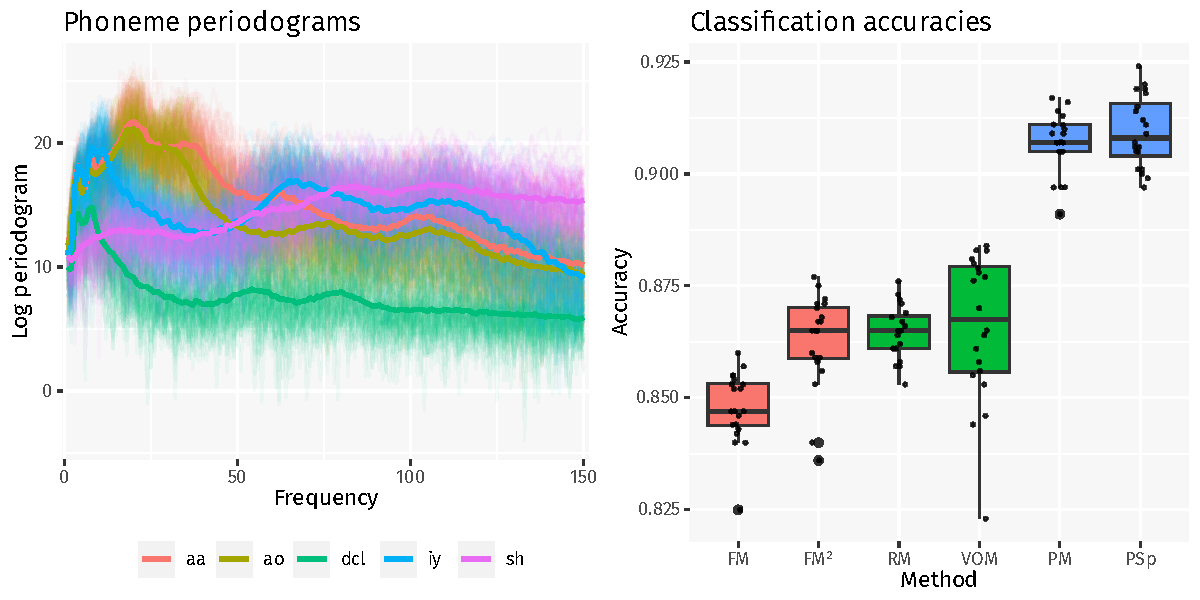
\includegraphics[width = \textwidth, page = 1]{phoneme}
    \caption{
        Classification of periodograms of digitized
        speech\protect\footnotemark, by phonemes (`aa', `ao', `dcl', `iy',
        `sh').
        The thick colored lines in the plot on the left mark the median curve
        across 400 examples in each of the five groups.
        The boxplot shows classification accuracies for 20 runs of each of the
        following methods: maximum depth classification using the first order
        (FM) and second order (FM$^2$) Fraiman-Muniz depths in red, the RM and
        VOM classifiers in green, and the maximum depth Mahalanobis (PM) and
        spatial (PSp) depth classifiers on $d$-variate feature vectors
        obtained by $d = 10$ random projections in blue.
        In each run, 50\% of the data was been aside for training.
    }
    \label{fig:phoneme_classification}
\end{figure}
\footnotetext{\url{http://www-stat.stanford.edu/ElemStatLearn}}



\subsection{Outlyingness matrices}

\textcite{dai-genton-2018} proposed a method which measures the outlyingness
of $\vx$ with respect to a population via depth as follows.

\begin{definition}
    Let $\vX$ be a $d$-variate stochastic process of continuous functions.
    At each time point $t \in [0, 1]$, the directional outlyingness is defined
    as
    \begin{equation}
        \vO(t) = \vO(\vX(t), F_{\vX(t)}) = \left(\frac{1}{D(\vX(t), F_{\vX(t)})} - 1\right)\, \vv(t),
    \end{equation}
    where $\vv(t)$ is the unit vector pointing from the median of $F_{\vX(t)}$
    to $\vX(t)$.
\end{definition}

\begin{definition}
    The functional directional outlyingness is defined as
    \begin{equation}
        \FO(\vX, F_{\vX}) = \int_{[0, 1]} \norm{\vO(t)}^2 \:w(t)\:dt.
    \end{equation}
\end{definition}

\begin{definition}
    \label{def:MO}
    The mean directional outlyingness is defined as
    \begin{equation}
        \MO(\vX, F_{\vX}) = \int_{[0, 1]} \vO(t) \:w(t)\:dt.
    \end{equation}
\end{definition}

\begin{definition}
    The variation of directional outlyingness is defined as
    \begin{equation}
        \VO(\vX, F_{\vX}) = \int_{[0, 1]} \norm{\vO(t) - \MO(t)}^2 \:w(t)\:dt.
    \end{equation}
\end{definition}

Here, $w$ is a weight function on $[0, 1]$.
In our discussion, we set $w = 1$.

It is easily verified that
\begin{equation}
    \FO^2 = \norm{\MO}^2 + \VO.
\end{equation}

\textcite{dai-genton-2018} propose using the $(d + 1)$-variate feature vectors
\begin{equation}
    \vY(\vX, F_{\vX}) = (\MO^\top,\, \VO)^\top
\end{equation}
corresponding to the curve $\vX$ for the purposes of classification.
The $\MO$ gives a sense of how outlying the curve $\vX$ is within $F_{\vX}$ as
a whole, while the $\VO$ measures the amount of variation in the outlyingness
over time.
Loosely speaking, $\MO$ is affected by the position, while $\VO$ is affected
by the shape of $\vX$ within $F_{\vX}$.
For instance, one may define the classifier
\begin{equation}
    \hat{\iota}(\vX) = \argmax_{1 \leq i \leq k} D'(\vY(\vX, F_i), F_{\vY(\vX, F_i)}),
\end{equation}
where $D'$ is a multivariate depth function.
This is simply a maximum depth classifier applied on the feature vectors
$\vY$.
When $D'$ is chosen to be the robust Mahalanobis depth, we have the RM
classifier
\begin{equation}
    \hat{\iota}_{RM}(\vX) = \argmax_{1 \leq i \leq k} D_{RM}(\vY(\vX, F_i), F_{\vY(\vX, F_i)}).
\end{equation}


\begin{definition}
    The functional directional outlyingness matrix is defined as
    \begin{equation}
        \FOM(\vX, F_{\vX}) = \int_{[0, 1]} \vO(t)\,\vO(t)^\top \:w(t)\:dt.
    \end{equation}
\end{definition}

\begin{definition}
    The functional directional outlyingness matrix is defined as
    \begin{equation}
        \VOM(\vX, F_{\vX}) = \int_{[0, 1]} (\vO(t) - \MO(t))\,(\vO(t) - \MO(t))^\top \:w(t)\:dt.
    \end{equation}
\end{definition}

Again, it is easily verified that
\begin{equation}
    \FOM = \MO\,\MO^\top + \VOM,
\end{equation}
and that
\begin{equation}
    \FO = \tr(\FOM), \qquad
    \VO = \tr(\VOM).
\end{equation}

We may also use the feature matrix $\VOM$, or its matrix norm $\norm{\VOM}_F$
corresponding to the curve $\vX$ for the purposes of classification.
Here, $\norm{\Cdot}_F$ denotes the Frobenius norm.
For instance, a $\VOM$ based classifier may be defined as
\begin{equation}
    \hat{\iota}_{\VOM}(\vX) = \argmin_{1 \leq i \leq k} \norm{\VOM(\vX, F_i)}_F.
\end{equation}



\subsection{Random projections}

Another approach is to use a feature vector consisting of multiple projections
of $\vX$.
Given functions $\vv_1, \dots, \vv_d$ chosen at random, we examine the
$d$-variate feature vectors
\begin{equation}
    \bm{V}(\vX, F_{\vX}) = \left(\ip{\vv_1}{\vX}, \dots, \ip{\vv_d}{\vX}\right)
\end{equation}
and apply a depth based multivariate classifier.
For instance, given a multivariate depth function $D'$, we may define a
classifier
\begin{equation}
    \hat{\iota}^d_{D'}(\vX) = \argmax_{1 \leq i \leq k} D'(\bm{V}(\vX, F_i), F_{\bm{V}(\vX, F_i)}).
\end{equation}


\section{Clustering}
\section{Outlier detection}

\section{Partially Observed Functional Data}


    \chapter{Local Depth Functions}
    

\begin{figure}
    \centering
    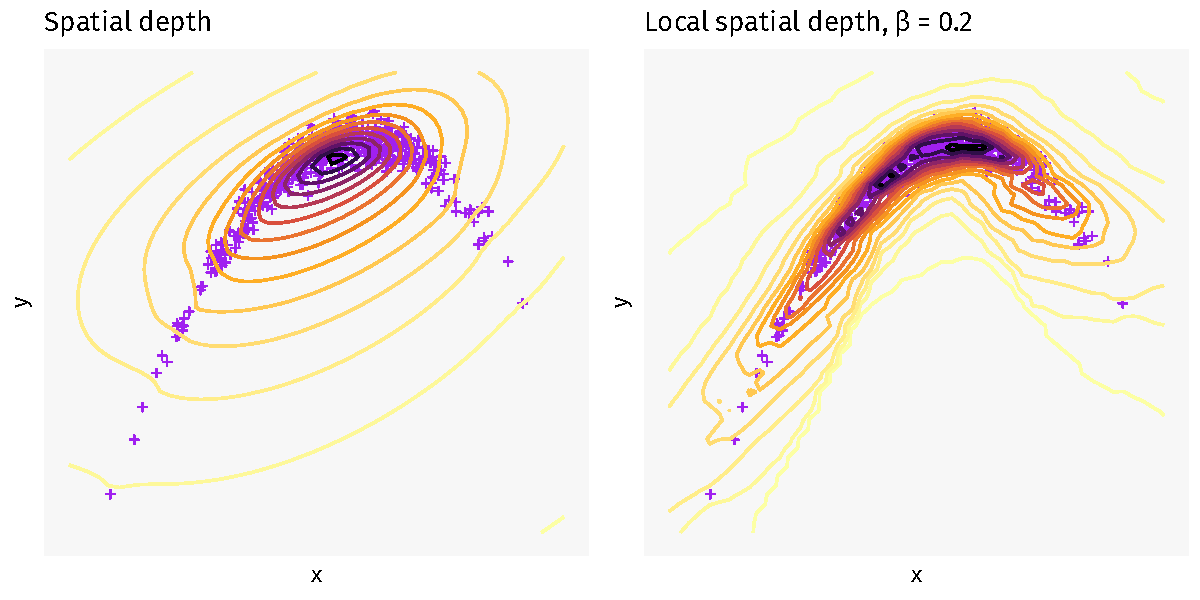
\includegraphics[width = \textwidth, page = 1]{localdepth_banana}
    \caption{
        Depth contours with respect to a `banana-shaped' distribution.
        Observe that the spatial depth contours fail to adequately capture the
        curved shape of the data cloud, in contrast with the local spatial
        depth (with $\beta = 0.2$) contours.
    }
    \label{fig:localdepth_banana}
\end{figure}


The depth functions which we've encountered so far are well suited for
unimodal, symmetric distributions.
For instance, depth functions like the halfspace and Mahalanobis depths behave
especially well with elliptical distributions: the depth and density contours
coincide.
These depth functions always produce convex, nested contours; the Zuo-Serfling
property \textbf{P3} also forces star-shaped central regions.
As a result, they may fail to capture the structure of distributions which are
not convexly supported (Figure~\ref{fig:localdepth_banana}), or those with
multiple modes (Figure~\ref{fig:localdepth_bimodal}).

Remedying this requires moving away from the \emph{global} structure to
\emph{local} structures of distributions.
One formulation of such a \emph{local depth} is due to
\textcite{agostinelli-romanazzi-2011}, where the halfspace and simplicial
depths are modified so as to capture only local information around a given
point $\vx \in \R^d$.
The local halfspace depth is obtained not by considering halfspaces containing
$\vx$ as in \ref{eq:halfspace}, but rather cuboidal slabs; similarly, the
local simplicial depth is defined by restricting the volumes of the random
simplices under consideration in \ref{eq:simplicial}.

In this chapter, we focus on the definition of \emph{local depth} and
\emph{local depth neighbourhoods} proposed by
\textcite{paindaveine-bever-2013}.
This allows the construction of a local counterpart of any existing global
depth function (multivariate, functional, or otherwise), giving it a distinct
advantage over the previous treatment.



\section{Local depth regions}

Given a distribution $F_{\vX}$, we may define a symmetrized distribution about
a point $\vx \in \mathscr{X}$ as
\begin{equation}
    F^{\vx}_{\vX} = \frac{1}{2}F_{\vX} + \frac{1}{2}F_{2\vx - \vX}. \label{eq:local_symmetrization}
\end{equation}
With this, $\vx$ becomes the point of central symmetry, hence the deepest
point in $F^{\vx}_{\vX}$ with respect to a depth function $D$ that obeys
\textbf{P2}.
Thus, the $\beta$-th central regions of $F^{\vx}_{\vX}$ behave like
neighbourhoods of $\vx$.

\begin{definition}[\cite{paindaveine-bever-2013}]
    The probability-$\beta$ depth-based neighbourhood of $\vx$ with respect to
    the distribution $F$ is defined as
    \begin{equation}
        N^{\vx}_\beta(F) = C_{F^{\vx}}(\beta),
    \end{equation}
    i.e.\ the $\beta$-th central region of $F$ symmetrized about $\vx$.
\end{definition}

When working with a sample $\mathscr{D} = \{\vX_i\}_{i = 1}^n$ from $F$, we
may obtain the $\beta$ depth-based neighbourhood of $\vx$ by first computing
the reflected sample $\mathscr{D}' = \{2\vx - \vX_i\}_{i = 1}^n$, then
arranging the elements of the symmetrized sample $\mathscr{D}^{\vx} =
\mathscr{D} \cup \mathscr{D}'$ in descending order by their empirical depth
values and choosing the first $\beta$ proportion of elements.
The neighbourhood $N^{\vx}_\beta(\hat{F}_n)$ is the convex hull of these
elements.


\begin{definition}[\cite{paindaveine-bever-2013}]
    \label{def:localdepth}
    Let $D$ be a depth function, and let $F^{\vx}_\beta$ denote the
    distribution $F$ conditional on the neighbourhood $N^{\vx}_\beta(F)$.
    The corresponding local depth function at locality level $\beta \in (0,
    1]$ is defined as
    \begin{equation}
        LD_\beta(\vx, F) = D(\vx, F^{\vx}_\beta)
    \end{equation}
\end{definition}

Again, when working with a sample $\mathscr{D} = \{\vX_i\}_{i = 1}^n$, we
obtain $LD_\beta(\vx, \hat{F}_n)$ by arranging the elements of $\mathscr{D}$
in descending order by their empirical depth values in the symmetrized sample
$\mathscr{D}^{\vx}$, choosing the first $\beta$ proportion of elements, and
computing the depth of $\vx$ with respect to these elements.

\begin{remark}
    When $\beta = 1$, the local depth $LD_1$ reduces to the original global
    depth $D$.
\end{remark}

\begin{remark}
    The notions of depth based neighbourhoods and local depth make sense for
    any distribution $F$ on a space $\mathscr{X}$ as long as the process of
    symmetrization around $\vx \in \mathscr{X}$ can be achieved.
\end{remark}


\begin{figure}
    \centering
    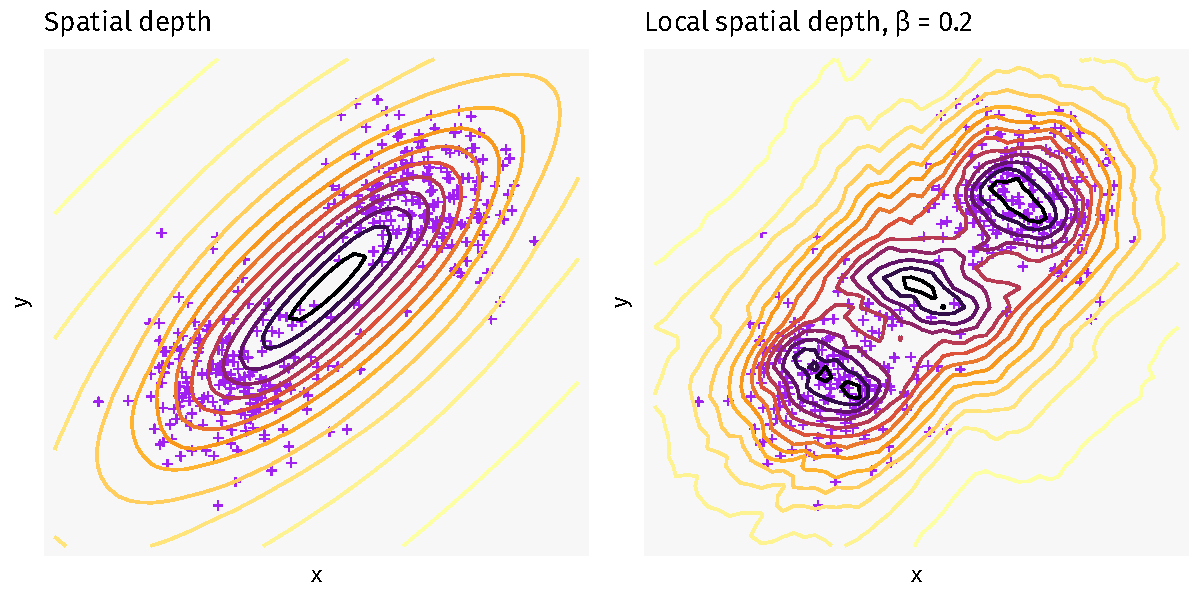
\includegraphics[width = \textwidth, page = 1]{localdepth_bimodal}
    \caption{
        Depth contours with respect to a bimodal distribution.
        Although the local spatial depth contours capture the two modes
        correctly, it erroneously ascribes high depth values to a region in
        between them.
    }
    \label{fig:localdepth_bimodal}
\end{figure}


\section{Regression based on local depth}
\label{sec:localdepth_regression}

\begin{figure}
    \centering
    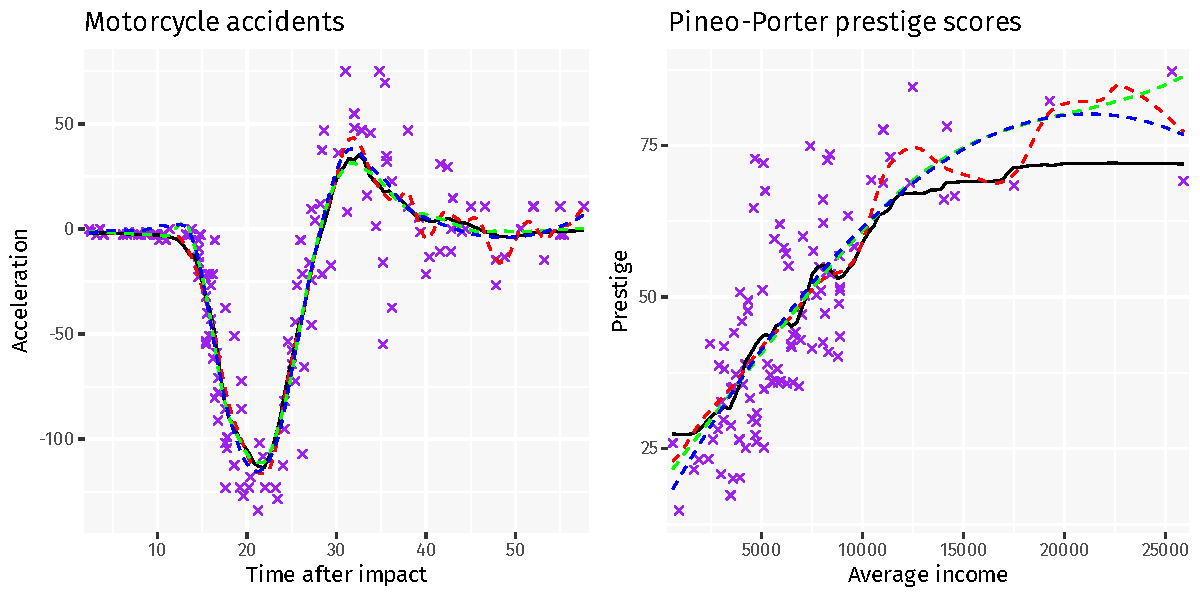
\includegraphics[width = \textwidth, page = 1]{localregression_univariate}
    \caption{
        Regression curves for the \texttt{cars} and \texttt{carData::Prestige}
        datasets available in R.
        The black curve indicates the local depth based estimate, the dashed
        red curve indicates the Nadaraya-Watson kernel based estimate, and the
        dashed green and blue curves indicate the local linear and quadratic
        estimates respectively.
        The locality levels and relevant bandwidths have been obtained by
        leave-one-out cross validation.
        The local depth based estimate is the best and second-best in terms of
        MSE respectively.
    }
    \label{fig:localregression_univariate}
\end{figure}


\begin{figure}
    \centering
    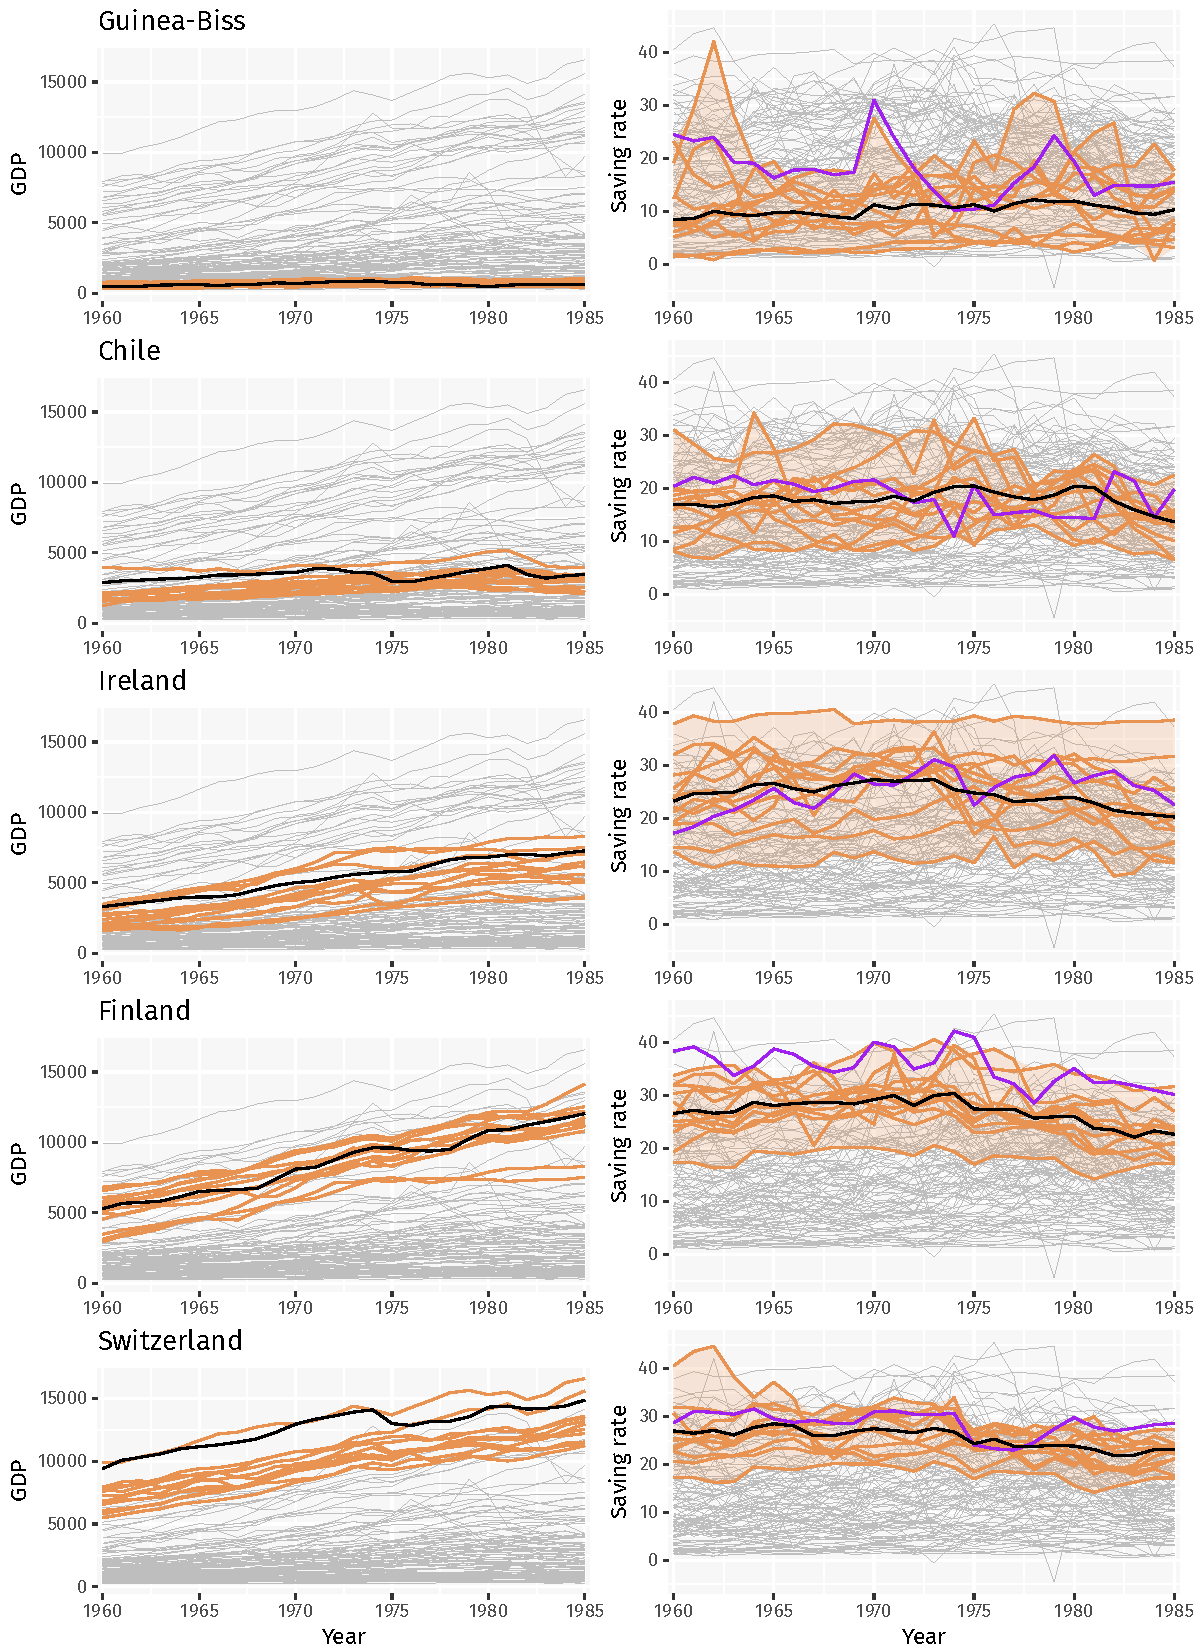
\includegraphics[width = \textwidth, page = 1]{localregression_penntable}
    \caption{
        Regression curves for the Penn table dataset, avaiable as
        \texttt{Ecdat::SumHes} in $R$.
        The covariates are GDP curves of different countries in the left
        column.
        The new GDP curve of the indicated country is marked in black, and its
        $\beta = 0.1$ neighbours are marked in orange.
        On the left, the estimated savings rate curve is marked in black, with
        the true curve in purple.
        The orange response curves correspond to the orange covariates, and
        their envelope is shaded in.
    }
    \label{fig:localregression_penn}
\end{figure}


\begin{definition}
    Let $D$ be a depth function, and let $\widetilde{F}^{\vx}_\beta$ denote
    the symmetrized distribution $F^{\vx}$ conditional on the neighbourhood
    $N^{\vx}_\beta(F)$.
    Given $\vx \in \mathscr{X}$, we may define a local depth kernel at
    locality level $\beta$ centered at $\vx$ as
    \begin{equation}
        K^{\vx}_\beta\colon N^{\vx}_\beta(F) \to \R, \qquad
        \vz \mapsto D(\vz, \widetilde{F}^{\vx}_\beta).
    \end{equation}
    This naturally extends to a map $\mathscr{X} \to \R$ as
    $K^{\vx}_\beta(\vz) = 0$ for $\vz \notin N^{\vx}_\beta(F)$.
\end{definition}

Note that $\widetilde{F}^{\vx}_\beta$ is angularly symmetric about $\vx$.
As a result, $K^{\vx}_\beta$ is maximized at and decreases away from $\vx$,
for reasonably well behaved depth functions (\textbf{P2} and \textbf{P3} for
multivariate depth functions).


With this, we propose the (linear) estimator
\begin{equation}
    \hat{\vy}_\beta(\vx) = \sum_i w_i(\vx)\, \vy_i, \qquad
    w_i(\vx) = \frac{K^{\vx}_\beta(\vx_i)}{\sum_j K^{\vx}_\beta(\vx_j)}.
    \label{eq:localregression}
\end{equation}
The locality level $\beta \in (0, 1]$ is a tuning parameter which may be
chosen via methods such as cross-validation.

The kernel function $K^{\vx}_\beta$ is supported on the neighbourhood
$N^{\vx}_\beta(F)$, whose shape may vary with changing $\vx \in \mathscr{X}$.
Indeed, since $N^{\vx}_\beta(\hat{F}_n)$ contains the $\beta$ proportion of
points from $\{\vx_i\}$ `closest' to $\vx$ (in the sense of being more central
in the symmetrized dataset $\mathscr{D}^{\vx}$), this neighbourhood ought to
be smaller when $\vx$ is more central, and larger when $\vx$ has fewer points
nearby.
Thus, $K^{\vx}_\beta$ behaves somewhat like a variable bandwidth or adaptive
kernel, whose shape adjusts to the surrounding data as $\vx$ varies.
Furthermore, the `bandwidth' of $K^{\vx}_\beta$ is controlled solely by the
parameter $\beta$ regardless of the dimensionality or nature of $\mathscr{X}$.
This stands in contrast with more traditional kernels which often require a
selection of multiple bandwidths.
For instance, a Gaussian kernel of the form
\begin{equation}
    \vz \mapsto \frac{1}{\prod_{i = 1}^d h_i} \exp\left(-\sum_i \frac{(x_i - z_i)^2}{2h_i^2}\right)
    \label{eq:kernel_gaussian}
\end{equation}
needs $d$ parameters $\{h_i\}_{i = 1}^d$ to be determined.

Equation~\ref{eq:localregression} may also be thought of as a weighted KNN
estimator, since $N^{\vx}_\beta(\hat{F}_n)$ always captures the same number of
points.

When the depth function $D$ is chosen to be affine invariant, the estimator
\ref{eq:localregression} is also affine invariant, in the sense that it is
unchanged by an affine transformation of $\mathscr{X}$.
This is because $N^{A\vx + \bm{b}}_\beta(F_{A\vX + \bm{b}})$ will simply be
the affine image of $N^{\vx}_\beta(F_{\vX})$.

The proposed estimator does however suffer from a lack of smoothness.
Additionally, it is fairly computationally expensive, since one must obtain
the symmetrized sample $\mathscr{D}^{\vx}$ for every $\vx$ where the estimate
is required.




    \chapter{Conclusion}
    

In conclusion, we have reviewed multiple realizations of depth functions in
the multivariate and functional settings, and seen numerous applications,
demonstrating the efficacy and versatility of this notion.
For a majority of these tasks, we have performed simulation studies,
reproduced results, and attempted to compare and contrast different procedures
proposed in the literature.
We have also tried to draw connections between different ideas; for instance,
the centrality-stability and MO-VO diagrams for functional outlier detection
(Section~\ref{sec:functional_outlier}) largely produce the same results, with
similar aims but differing approaches.
The use of random projections in functional data classification
(Section~\ref{sec:functional_classification_RP}) draws inspiration from the
random Tukey depth \parencite{albertos-reyes-2008a}, the $J$-th order depths
\parencite{nagy-gijbels-hlubinka-2017}, and the Cramer-Wold device in Hilbert
spaces \parencite{albertos-fraiman-ransford-2007}.
We have also attempted to propose a new method of regression
(Section~\ref{sec:localdepth_regression}) using the local depth regions of
\textcite{paindaveine-bever-2013}; further study into its theoretical
consistency as well as results from simulations are merited.

One area which we have not covered in much detail is regression.
For instance, \textcite{zuo-2021} gives an overview of depths used in the
context of linear regression.
\textcite{chowdhury-chaudhuri-2019} explore quantile regression for functional
data using spatial depth.
This uses the language of spatial quantiles
\parencite{chakraborty-chaudhuri-2014b}, where the spatial $\vu$-quantile
$\bm{Q}(\vu)$ for $\vu \in B^*(\bm{0}, 1) \subset \mathscr{X}^*$ is the
minimizer of
\begin{equation}
    \E_{\vX \sim F}\left[\norm{\bm{Q} - \vX} - \norm{\vX}\right] - \vu(\bm{Q}).
\end{equation}

The code used to produce this document, its figures, and results can be found
in this thesis' GitHub
repository\footnote{\url{https://github.com/sahasatvik/ms-thesis}}.



    \nocite{*}
    \printbibliography

    \appendix


\end{document}
